\documentclass{beamer}

\usepackage{qtree}

\usepackage{beamerthemetree}
\usepackage{color}
\setbeamertemplate{footline}[frame number]
\usepackage{graphicx}
%\usepackage{xyling}
%\usepackage[swedish]{babel} 
\usepackage[latin1]{inputenc} 
\usepackage{natbib}
\renewcommand{\newblock}{}
\usepackage{hyperref}


\title{Grammar in TTR: frames and lexical semantics; Incremental context and content; Tense and aspect\ignore{\thanks{This research was supported in part by VR project 2009-1569, Semantic
analysis of interaction and coordination in dialogue (SAICD).}}}
\author{Robin Cooper\\ 
University of Gothenburg\\Jonathan Ginzburg\\
Universit\'e Paris-Diderot, Sorbonne Paris-Cit\'e}
\date{Type theory with records for natural language semantics, NASSLLI
2012 \\ Lecture 2}

\AtBeginSection[]
{
   \begin{frame}[plain]
       \frametitle{Outline}
       \tableofcontents[currentsection]
   \end{frame}
}

\newcommand{\backgroundyellow}{\beamertemplateshadingbackground{yellow!40}{magenta!20}}
\newcommand{\backgroundwhite}{\beamertemplateshadingbackground{white!100}{white!100}}

\newcommand{\ignore}[1]{}

\newenvironment{display}{\begin{center}}{\end{center}}

%
% Reference the next example in the text:
%
\newcommand{\nexteg}[1]{\addtocounter{examplectr}{1}(\arabic{examplectr}{#1})\addtocounter{examplectr}{-1}}
%
% Reference the previous example in the text:
%
\newcommand{\preveg}[1]{(\arabic{examplectr}{#1})}
%
% Reference examples by relative offsets:
%
\newcommand{\egnum}[2]{\addtocounter{examplectr}{#1}(\arabic{examplectr}{#2})\addtocounter{examplectr}{-#1}}
%
%
% ENVIRONMENTS
%
% Examples Environments
%
\newcounter{examplectr}
\newcounter{subexamplectr}[examplectr]
\renewcommand{\thesubexamplectr}{\alph{subexamplectr}}
%
% Sub-example Macro:
%
\newenvironment{subex}%
   {%\vspace*{-.8\baselineskip}
     \begin{list}
       {\alph{subexamplectr}.}%
       {\setlength{\topsep}{0in}
        \setlength{\leftmargin}{1em}%{0.25in}
        %\setlength{\listparindent}{-2em}
        %\setlength{\labelsep}{\baselineskip}
 \usecounter{subexamplectr} }
       }%
   {\end{list}}
%
% Single Example Macro
%
\newenvironment{ex}%
   { \refstepcounter{examplectr}
     
\bigskip

    % \begin{list}
      % {
       (\arabic{examplectr})%}%
       % {%\setlength{\topsep}{0in}
%         \setlength{\leftmargin}{4em}%{0.75in}
%         \setlength{\labelsep}{\baselineskip}
% }
        \hspace*{1em}\begin{minipage}[t]{4in} 
%\item
   }%
   {\end{minipage}

\bigskip

    %\end{list}
}
%
% End of example macro
%

\newcommand{\subegref}[2]{(\ref{#1}\ref{#2})}

\newcommand{\beg}{\begin{ex}}
\newcommand{\eeg}{\end{ex}}
\newcommand{\bseg}{\begin{subex}}
\newcommand{\eseg}{\end{subex}}


\newcommand{\egstack}[1]{\begin{tabular}[t]{@{}l@{}} #1 \\ \\
  \end{tabular}}

%Records

\newcommand{\record}[1]{$\left[\mbox{\begin{tabular}{lcl} #1
\end{tabular}}\right]$} 
\newcommand{\smallrecord}[1]{$\left[\mbox{\begin{tabular}{@{}l@{}c@{}l@{}} #1
\end{tabular}}\right]$}

\newcommand{\field}[2]{#1 & = & #2}
\newcommand{\tfield}[2]{#1 & : & #2}
\newcommand{\smalltfield}[2]{#1:#2 & &}
\newcommand{\mfield}[3]{#1=#2 & : & #3}
\newcommand{\smallmfield}[3]{#1=#2:#3 & &}
\newcommand{\hfield}[2]{{\sc #1} & & #2}



\begin{document}

\frame[plain]{\titlepage}
\frame[plain]{\frametitle{Outline}\tableofcontents}

\section{Frames in lexical semantics \citep{Cooper2010,Cooper2012}}

\frame{

\frametitle{The content of \textit{ran}}

\begin{itemize}

\item $\lambda r$:\smallrecord{\smalltfield{x}{\textit{Ind}}}(\record{\tfield{e-time}{\textit{Time}} \\
        \tfield{c$_{\mathrm{tns}}$}{e-time.end$<\iota$.start} \\
        \tfield{c$_{\mathrm{run}}$}{run($r$.x,e-time)}})

\pause \item Frames as arguments

\pause \item This is an individual level verb phrase interpretation, even though it
takes a frame as argument, the predicate `run' takes an individual as argument.

\end{itemize}


}

\frame{

\frametitle{\textit{rises} -- a predicate of frames}

\begin{itemize}

\item $\lambda r$:\smallrecord{\smalltfield{x}{\textit{Ind}}}(\record{\tfield{e-time}{\textit{TimeInt}} \\
        \tfield{c$_{\mathrm{tns}}$}{e-time$=\iota$} \\
        \tfield{c$_{\mathrm{run}}$}{rise($r$,e-time)}})

\pause \item This is a frame level verb phrase interpretation, the
predicate `rise' takes a frame as argument

\pause \item \textit{The temperature is rising, the temperature is
  ninety} $\not\Rightarrow$ \textit{Ninety is rising}

\pause \item  What can it mean for a frame to rise?

\end{itemize}

}

\frame{

\frametitle{The record type \textit{AmbTemp}}

\begin{itemize}
\item \record{\tfield{x}{\textit{Ind}} \\
        \tfield{e-time}{\textit{Time}} \\
        \tfield{e-location}{\textit{Loc}} \\
        \tfield{c$_{\mathrm{temp\_at\_in}}$}{temp\_at\_in(e-time, e-location, x)}}

\pause \item a record of this type will meet the following two conditions:
\begin{itemize} 
 
\item it will contain \textit{at least} fields with the same labels as
  the type (it may contain more) 
 
\pause \item each field in the record with the same label as a field in the
  record type will contain an object of the type in the
  corresponding field of the record type.  (Any additional fields with
  different labels to those in the record type may contain objects of
  any type.)
\end{itemize}

\end{itemize}
}

\frame{

\frametitle{The type \textit{TempRise}}

\smallrecord{\smalltfield{e-time}{\textit{TimeInt}} \\
        \smalltfield{start}{ 
\smallrecord{\smalltfield{x}{\textit{Ind}} \\
        \smallmfield{e-time}{e-time.start}{\textit{Time}} \\
        \smalltfield{e-location}{\textit{Loc}} \\
        \smalltfield{c$_{\mathrm{temp\_at\_in}}$}{temp\_at\_in(start.e-time,
          start.e-location, start.x)}}
} \\
       \smalltfield{end}{
\smallrecord{\smalltfield{x}{\textit{Ind}} \\
        \smallmfield{e-time}{e-time.end}{\textit{Time}} \\
        \smallmfield{e-location}{start.e-location}{\textit{Loc}} \\
        \smalltfield{c$_{\mathrm{temp\_at\_in}}$}{temp\_at\_in(end.e-time,
          end.e-location, end.x)}}
} \\
       \smallmfield{event}{start$^{\frown}$end}{\textit{AmbTemp}$^{\frown}$\textit{AmbTemp}}
       \\
       \smalltfield{c$_{\mathrm{incr}}$}{start.x$<$end.x}}

\bigskip

\pause If $r$:\textit{AmbTemp} and $i$:\textit{TimeInt} then
$e$:rise($r$,$i$) iff $e$:\textit{TempRise}, $e$.start=$r$ and $e$.e-time=$i$.

}

\frame{

\frametitle{Does \textit{rise} have a general meaning?}

At this level of detail, the type of an event of a price rise is
slightly different.

}

\frame{

\frametitle{The type \textit{PriceRise}}

\smallrecord{\smalltfield{e-time}{\textit{TimeInt}} \\
        \smalltfield{start}{ 
\smallrecord{\smalltfield{x}{\textit{Ind}} \\
        \smallmfield{e-time}{e-time.start}{\textit{Time}} \\
        \smalltfield{e-location}{\textit{Loc}} \\
        \smalltfield{commodity}{\textit{Ind}} \\
        \smalltfield{c$_{\mathrm{price\_of\_at\_in}}$}{price\_of\_at\_in(start.commodity,\\
\hspace*{8em}start.e-time,
          start.e-location, start.x)}}
} \\
       \smalltfield{end}{
\smallrecord{\smalltfield{x}{\textit{Ind}} \\
        \smallmfield{e-time}{e-time.end}{\textit{Time}} \\
        \smallmfield{e-location}{start.e-location}{\textit{Loc}} \\
        \smallmfield{commodity}{start.commodity}{\textit{Ind}} \\
        \smalltfield{c$_{\mathrm{price\_of\_at\_in}}$}{price\_of\_at\_in(end.commodity,\\
\hspace*{8em}end.e-time,
          end.e-location, end.x)}}
} \\
       \smallmfield{event}{start$^{\frown}$end}{\textit{Price}$^{\frown}$\textit{Price}}
       \\
       \smalltfield{c$_{\mathrm{incr}}$}{start.x$<$end.x}}

}

\frame{

\frametitle{\textit{The Titan rises}}

(description of a video game)

\bigskip

As they get to deck, they see the Inquisitor, calling out to a Titan
in the seas. \textbf{The giant Titan rises through the waves}, shrieking at the
Inquisitor. 

}

\frame{

\frametitle{The type \textit{LocRise}}

\smallrecord{\smalltfield{e-time}{\textit{TimeInt}} \\
        \smalltfield{start}{ 
\smallrecord{\smalltfield{x}{\textit{Ind}} \\
        \smallmfield{e-time}{e-time.start}{\textit{Time}} \\
        \smalltfield{e-location}{\textit{Loc}} \\
        \smalltfield{c$_{\mathrm{at}}$}{at(start.x,start.e-location,start.e-time)}}
} \\
       \smalltfield{end}{
\smallrecord{\smallmfield{x}{start.x}{\textit{Ind}} \\
        \smallmfield{e-time}{e-time.end}{\textit{Time}} \\
        \smalltfield{e-location}{\textit{Loc}} \\
         \smalltfield{c$_{\mathrm{at}}$}{at(end.x,end.e-location,end.e-time)}}
} \\
       \smallmfield{event}{start$^{\frown}$end}{\textit{Position}$^{\frown}$\textit{Position}}
       \\
       \smalltfield{c$_{\mathrm{incr}}$}{height(start.e-location)$<$height(end.e-location)}}

}

\frame{

\frametitle{Semantic coordination}

(Work with Staffan Larsson: \citealp{Larsson2007,CooperLarsson2009,LarssonCooper2009})

\bigskip

Instead of  ``What is the meaning of expression $E$?''

\medskip

\pause we propose

\begin{description}

\item[the coordination question] Given resources $R$, how can
agent $A$ construct a meaning for a particular utterance $U$ of
expression $E$?

\pause \item[the resource update question] What effect will this have
on $A$'s resources $R$?

\end{description}

}



\section{Grammar rules as dependent event types \citep{Cooper2012}}

\frame{

\frametitle{Fernando's string theory}

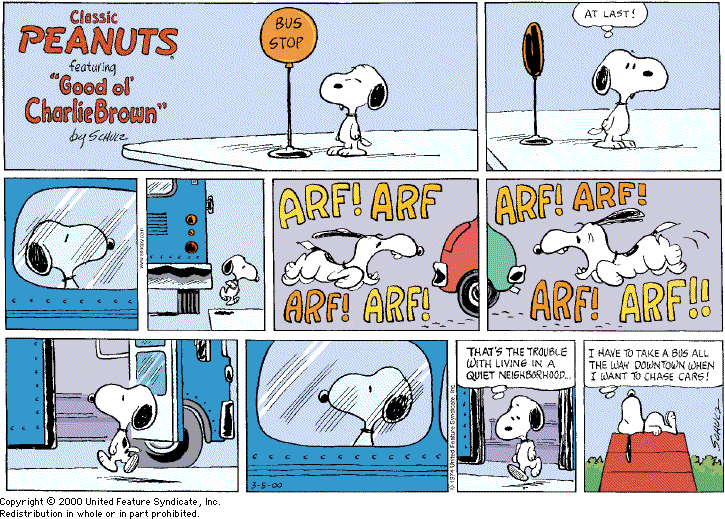
\includegraphics[width=.9\textwidth]{snoopy}

}

\frame{

\frametitle{A Fernando finite automaton representation}

\framebox{wait-at-busstop}$^*$\ \framebox{bus-arrive}\
\fbox{get-on-bus}\ \fbox{travel-on-bus}\ \fbox{get-off-bus}\ \framebox[1em]{}$^+$

}

% \frame{

% \frametitle{Regular types}



% \begin{enumerate} 
 
% \item if $T_1$, $T_2$ $\in$ {\bf Type}, then ${T_1}^\frown\!T_2$ $\in$ {\bf Type}

% $a : {T_1}^\frown\!T_2$ iff $a=x^\frown\!y$, $x:T_1$ and $y:T_2$
 
% \item if $T$ $\in$ {\bf Type} then $T^+$ $\in$ {\bf Type}.

% $a:T^+$ iff $a=x_1^\frown\!\ldots^\frown\!x_n$, $n>0$ and for $i$, $1\leq
% i\leq n$, $x_i:T$ 

% \ldots
 
% \end{enumerate} 

% }

\frame{

\frametitle{String types and finite automata}

\begin{itemize} 
 
\item \textit{bus-trip}=
\textit{get-bus}$^\frown$\textit{travel-on-bus}$^\frown$\textit{get-off-bus} 
 
\pause\item \textit{get-bus} = \textit{wait-at-busstop}$^{*\frown}$\textit{bus-arrive}$^\frown$\textit{get-on-bus}
 
\end{itemize} 

\pause or in Fernando's kind of notation:

\begin{itemize} 
 
\item $\mathcal{L}$(\textit{bus-trip})=
$\mathcal{L}$(\textit{get-bus})$^\frown$$\mathcal{L}$(\textit{travel-on-bus})$^\frown$$\mathcal{L}$(\textit{get-off-bus})
 
\item $\mathcal{L}$(\textit{get-bus}) = $\mathcal{L}$(\textit{wait-at-busstop})$^{*\frown}$$\mathcal{L}$(\textit{bus-arrive})$^\frown$$\mathcal{L}$(\textit{get-on-bus})
 
\end{itemize}

where $L_1^{\frown}L_2 = \{a^{\frown}b\mid a\in L_1\ \mathrm{and}\ b\in L_2\}$

}

%\frame{

% \frametitle{Or maybe dependent regular types}

% \begin{itemize} 
 
% \item \textit{bus-trip}($A,B$)=
% \textit{get-bus}($A$)$^\frown$\textit{travel-on-bus}$^\frown$\textit{get-off-bus}($B$) 
 
% \item \textit{get-bus}($A$) =
%   \textit{wait-at-busstop}($A$)$^{*\frown}$\textit{bus-arrive}($A$)$^\frown$\textit{get-on-bus}($A$)

% \pause \item \textit{return-bus-trip}($A,B$) =
%   \textit{bus-trip}($A,B$)$^\frown$\textit{Event}$^{+\frown}$\textit{bus-trip}($B,A$)

% % \pause \item an agent who can organize non-linguistic events in this
% % way should be able to do something similar with linguistic events

 
% \end{itemize}
  
% }



% \frame{

% \frametitle{A game of fetch}

 
 
% 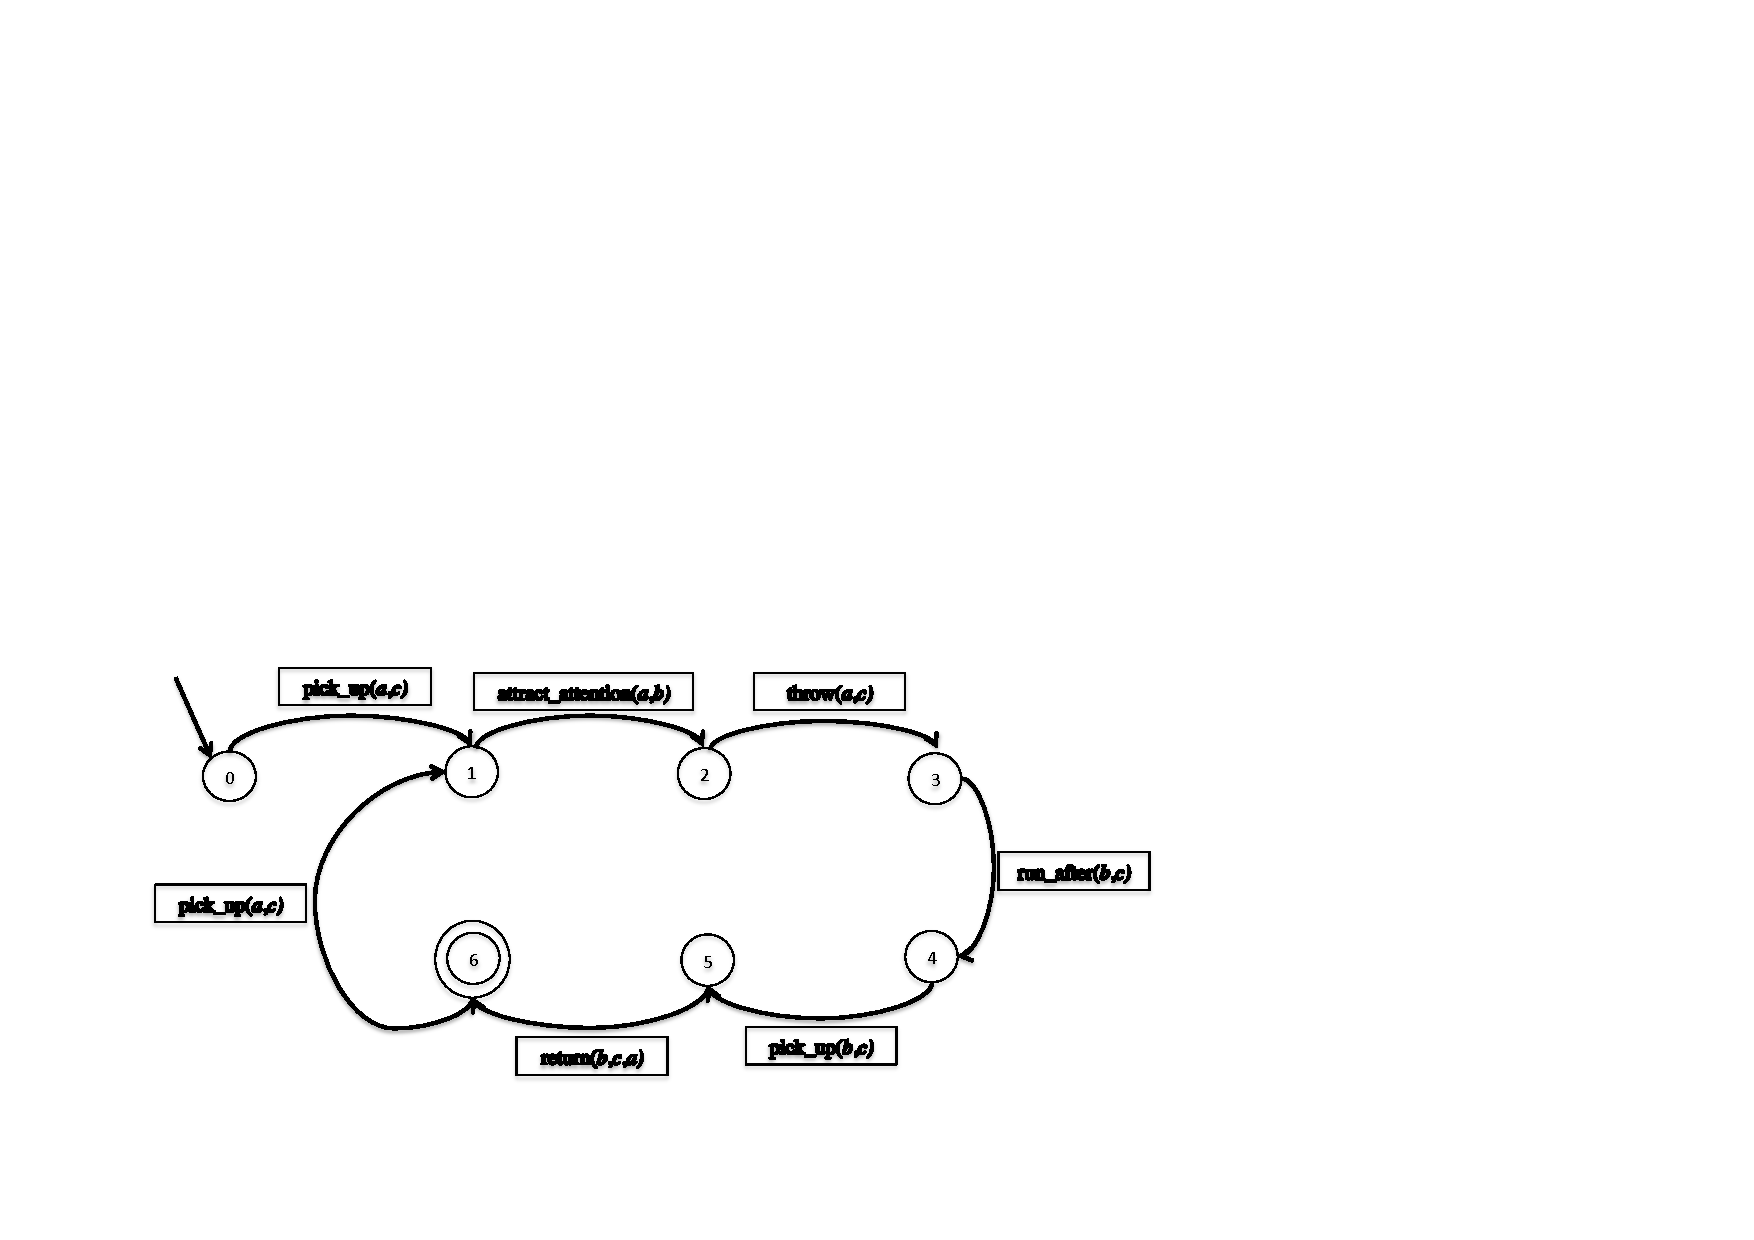
\includegraphics[width=\textwidth]{fetch-fs} 
 
% \pause(pick\_up($a$,$c$)$^{\frown}$attract\_attention($a$,$b$)$^{\frown}$throw($a$,$c$)$^{\frown}$run\_after($b$,$c$)$^{\frown}$
% \\ \hspace*{1ex}pick\_up($b$,$c$)$^{\frown}$return($b$,$c$,$a$))$^+$ 
 

  

% }

% \frame{

% \frametitle{Getting serious about time: intervals}

% \record{\tfield{start}{\textit{Time}} \\
%         \tfield{end}{\textit{Time}} \\
%         \tfield{c$_<$}{start$<$end}}

% }

% \frame{

% \frametitle{Getting serious about time: the fetch-game type}

% (\smallrecord{\smalltfield{e-time}{\textit{TimeInt}} \\
%              \smalltfield{c$_{\mathrm{pick\_up}}$}{pick\_up($a$,$c$,e-time)}}$^{\frown_\leq}$\smallrecord{\smalltfield{e-time}{\textit{TimeInt}}
%              \\
%                   \smalltfield{c$_{\mathrm{att\_att}}$}{attract\_attent($a$,$b$,e-time)}}$^{\frown_\leq}$

% \medskip
% \smallrecord{\smalltfield{e-time}{\textit{TimeInt}} \\
%              \smalltfield{c$_{\mathrm{throw}}$}{throw($a$,$c$,e-time)}}$^{\frown_\leq}$\smallrecord{\smalltfield{e-time}{\textit{TimeInt}} \\
%              \smalltfield{c$_{\mathrm{run\_after}}$}{run\_after($b$,$c$,e-time)}}$^{\frown_\leq}$

% \medskip
% \smallrecord{\smalltfield{e-time}{\textit{TimeInt}} \\
%              \smalltfield{c$_{\mathrm{pick\_up}}$}{pick\_up($b$,$c$,e-time)}}$^{\frown_\leq}$\smallrecord{\smalltfield{e-time}{\textit{TimeInt}} \\
%              \smalltfield{c$_{\mathrm{return}}$}{return($b$,$c$,$a$,e-time) }})$^{+_\leq}$
% }

% \frame{

% \frametitle{Temporal concatenation}

% \begin{enumerate} 
% \item If $T_1$ and $T_2$ are subtypes of
% \smallrecord{\smalltfield{e-time}{\textit{TimeInt}}}$^+$ then
% $T_1^{\frown_\leq}T_2$ is a type. 

% \item $a:T_1^{\frown_\leq}T_2$ iff $a=a_1^{\frown}a_2$, $a_1:T_1$, $a_2:T_2$ and
%   last($a_1$).e-time.end$\leq$first($a_2$).e-time.start
% \end{enumerate}

% }

% \frame{

% \frametitle{Temporal Kleene-+}

% \begin{enumerate} 
 
% \item If $T$ is a subtype of
%   \smallrecord{\smalltfield{e-time}{\textit{TimeInt}}} then $T^{+_\leq}$
%   is a type
 
% \item $a:T^{+_\leq}$ iff $a=x_1^\frown\!\ldots^\frown\!x_n$, $n>0$ and
%   for $i$, $j$, $1\leq
% i<j\leq n$, $x_i:T$, $x_j:T$ and $x_i^{\frown}x_j:T^{\frown_\leq}T$ 
 
% \end{enumerate}

% }

% \frame{

% \frametitle{Gapless temporal concatenation}

% \begin{enumerate} 
% \item If $T_1$ and $T_2$ are subtypes of
% \smallrecord{\smalltfield{e-time}{\textit{TimeInt}}}$^+$ then
% $T_1^{\frown_{\leq=}}T_2$ is a type. 

% \item $a:T_1^{\frown_{\leq=}}T_2$ iff $a=a_1^{\frown}a_2$, $a_1:T_1$, $a_2:T_2$ and
%   last($a_1$).e-time.end$=$first($a_2$).e-time.start
% \end{enumerate}

% }

% \frame{

% \frametitle{Gapless temporal Kleene-+}

% \begin{enumerate} 
 
% \item If $T$ is a subtype of
%   \smallrecord{\smalltfield{e-time}{\textit{TimeInt}}} then $T^{+_{\leq=}}$
%   is a type
 
% \item $a:T^{+_{\leq=}}$ iff $a=x_1^\frown\!\ldots^\frown\!x_n$, $n>0$ and
%   for $i$, $j$, $1\leq
% i<j\leq n$, $x_i:T$, $x_j:T$ and $x_i^{\frown}x_j:T^{\frown_{\leq=}}T$ 
 
% \end{enumerate}

% }



\frame{

\frametitle{Two kinds of partiality}
\begin{itemize} 
 
\item not all frames are perceived -- infer more 
 
\pause \item  individual frame type partially specified

\pause \item \record{\tfield{x}{\textit{Ind}} \\
                     \tfield{y}{\textit{Ind}} \\
                     \tfield{c$_1$}{bus-stop(y)} \\
                     \tfield{c$_2$}{near(x,y)} \\
                     \tfield{c$_3$}{wait-for(x,\record{\tfield{x}{\textit{Ind}}\\
                                                       \tfield{c$_1$}{bus(x)}
                                                       \\
                                                       \tfield{c$_2$}{arrive-at(x,y)}})}}

\end{itemize}

}

% \backgroundyellow 

% \frame{

% \frametitle{Official notation}


 
%  \smallrecord{\smalltfield{x}{\textit{Ind}} \\
%                      \smalltfield{y}{\textit{Ind}} \\
%                      \smalltfield{c$_1$}{$\langle\lambda
%                        v$:\textit{Ind}(bus-stop(v)),$\langle$y$\rangle\rangle$} \\
%                      \smalltfield{c$_2$}{$\langle\lambda
%                        v_1$:\textit{Ind}($\lambda
%                        v_2$:\textit{Ind}(near($v_1$,$v_2$))), $\langle$x,y$\rangle\rangle$} \\
%                      \smalltfield{c$_3$}{$\langle\lambda
%                        v_1$:\textit{Ind}($\lambda v_2$:\textit{Ind}(\\
% \hspace*{2em}wait-for($v_1$,\smallrecord{\smalltfield{x}{\textit{Ind}}\\
%                                                        \smalltfield{c$_1$}{$\langle\lambda
%                                                          v$:\textit{Ind}(bus($v$)),$\langle$x$\rangle\rangle$}
%                                                        \\
%                                                        \smalltfield{c$_2$}{$\langle\lambda
%                                                          v$:\textit{Ind}(arrive-at($v$,$v_2$)),$\langle$x$\rangle\rangle$}})),
%                                                    $\langle$x,y$\rangle\rangle$)}}

% } 

% \backgroundwhite

\frame{

\frametitle{Specification with Snoopy}
\record{\mfield{x}{\textcolor{red}{snoopy}}{\textit{Ind}} \\
                     \tfield{y}{\textit{Ind}} \\
                     \tfield{c$_1$}{bus-stop(y)} \\
                     \tfield{c$_2$}{near(x,y)} \\
                     \tfield{c$_3$}{wait-for(x,\record{\tfield{x}{\textit{Ind}}\\
                                                       \tfield{c$_1$}{bus(x)}
                                                       \\
                                                       \tfield{c$_2$}{arrive-at(x,y)}})}}

\bigskip

What are \textit{manifest fields} \record{\mfield{$\ell$}{$a$}{$T$}}?

}

\frame{

\frametitle{Manifest fields}

 \record{\mfield{$\ell$}{$a$}{$T$}}

is a convenient notation for

\record{\tfield{$\ell$}{$T_a$}}


\medskip

If $a:T$, then $T_a$ is a type (the \textit{singleton type of $a$}).

$b:T_a$ iff $b=a$

}

\frame{

\frametitle{Partial perception of linguistic events}

\begin{itemize} 
 
\item perceive phonology (or phonetics)
 
\item infer syntax/semantics 
 
\end{itemize} 

} 

\frame{

\frametitle{Grammar rules}

Grammar rules are of the form

\medskip

$\lambda s_1:T_1\ldots\lambda s_n:T_n(T)$

\medskip

where $T_i$ and $T$ are \textit{sign types}. 

\bigskip

Sign types correspond to the notion of sign in HPSG. 

}

\frame{

\frametitle{The type \textit{Sign}}

\record{\tfield{s-event}{\textit{SEvent}}
                               \\
        \tfield{synsem}{\record{\tfield{cat}{\textit{Cat}}\\
                                \tfield{cnt}{\textit{Cnt}}}}}

\bigskip

But what are \textit{SEvent}, \textit{Cat} and \textit{Cnt}?

}

\frame{

\frametitle{The type \textit{SEvent}}

\record{\tfield{phon}{\textit{Phon}}\\
                                 \tfield{s-time}{\record{\tfield{start}{\textit{Time}}
                                     \\
                                                         \tfield{end}{\textit{Time}}}}\\
                                 \tfield{utt$_\mathrm{at}$}{uttered\_at(phon,
                                   s-time.start,
                                   s-time.end)}}

\bigskip

A minimal solution, from \cite{Cooper2012}.

}

\frame{

\frametitle{The type \textit{SEvent}, a more refined type}

\record{\tfield{e-time}{\textit{TimeInt}} \\
        \tfield{e-loc}{\textit{Loc}} \\
        \tfield{sp}{\textit{Ind}} \\
        \tfield{au}{\textit{Ind}} \\
        \tfield{phon}{\textit{Phon}} \\
        \tfield{e}{utter(sp,phon,au,e-time,e-loc)}}

\bigskip

However, this may not always be correct:  more than one person may be
in the audience;  more than one person may collaborate on a single
speech event - \textit{split utterances}.


}

\frame{

\frametitle{The type \textit{Cat}}

s, np, vp, n$_{\mathrm{prop}}$, v$_{\mathrm{i}}$ : \textit{Cat}

\bigskip

There will be more in a more extensive fragment.

}

\frame{

\frametitle{The type \textit{Cnt}}

\textit{RecType}$\vee$(\textit{Ppty}$\vee$\textit{Quant})

\bigskip

There will be more in a more extensive fragment

\bigskip

\pause If $T_1$, $T_2$ are types, then $T_1\vee T_2$ is a type (the
\textit{join} of $T_1$ and $T_2$).

$a:T_1\vee T_2$ iff either $a:T_1$ or $a:T_2$

\bigskip

\pause \textit{Ppty}, ``property'' is to be
\smallrecord{\smalltfield{x}{\textit{Ind}}}$\rightarrow$\textit{RecType}

(cf. $\langle e,t\rangle$)

\bigskip

\pause \textit{Quant}, ``quantifier'' is to be
\textit{Ppty}$\rightarrow$\textit{RecType} 

(cf. $\langle\langle e,t\rangle, t\rangle$)

}

\frame{

\frametitle{The lexicon: Proper names}

If $W$ is
a phonological type such as ``Sam'' or ``John'' and $a$:\textit{Ind},
lex$_{\mathrm{n}_\mathrm{Prop}}$($W,a$) is

\medskip

\textit{Sign} \d{$\wedge$} \\
\record{\tfield{s-event}{\record{\tfield{phon}{\textit{W}}}} \\
        \tfield{synsem}{\record{\mfield{cat}{n$_{\mathrm{Prop}}$}{\textit{Cat}} \\
                                \mfield{cnt}{$\lambda
                                  v$:\textit{Ppty}($v$(\smallrecord{\field{x}{$a$}}))}{\textit{Quant}}}}}

\bigskip

$T_1$\d{$\wedge$}$T_2$ is the \textit{merge} of the two types
$T_1$,$T_2$.  If at least on of the two types is not a record type it
is identical with the meet $T_1\wedge T_2$.  So what is the meet of
two types and the merge of two record
types?






}

\frame{

\frametitle{Meets and merges}

If $T_1$,$T_2$ are types, then $T_1\wedge T_2$ is a type (the
\textit{meet} of $T_1$ and $T_2$).

$a:T_1\wedge T_2$ iff $a:T_1$ and $a:T_2$

\bigskip

The basic idea of \textit{merge}  (full definition in
\citealp{Cooper2012}):

\smallrecord{\smalltfield{f}{$T_1$}}\d{$\wedge$}{\smallrecord{\smalltfield{g}{$T_2$}}}
  = \smallrecord{\smalltfield{f}{$T_1$} \\
                 \smalltfield{g}{$T_2$}}


\smallrecord{\smalltfield{f}{$T_1$}}\d{$\wedge$}{\smallrecord{\smalltfield{f}{$T_2$}}}
  = \smallrecord{\smalltfield{f}{$T_1$\d{$\wedge$}$T_2$}}

\medskip cf. unification


}

\frame{

\frametitle{The lexicon: intransitive verbs (individual level)}

If $W$ is
a phonological type like ``run'' or ``walk'' and $p$ is a predicate with arity $\langle$\textit{Ind},\textit{TimeInt}$\rangle$,
lex$_{\mathrm{V_{\mathrm{i}}}}$($W,p$) is

\textit{Sign} \d{$\wedge$} \\
\smallrecord{\smalltfield{s-event}{\smallrecord{\smalltfield{phon}{\textit{$W$}}}} \\
        \smalltfield{synsem}{\smallrecord{\smallmfield{cat}{v$_{\mathrm{i}}$}{\textit{Cat}} \\
                                \smallmfield{cnt}{$\lambda
                                  r$:\smallrecord{\smalltfield{x}{\textit{Ind}}}
                                  (\smallrecord{\smalltfield{e-time}{\textit{TimeInt}}
                                    \\
                                           \smalltfield{c$_W$}{$p$($r$.x,e-time)}})}{\textit{Ppty}}}}}


}

\frame{

\frametitle{Composition rules as dependent types}

\begin{description}
\item[unary rules] $\lambda s:T_1(T_2)$, where
  $T_1,T_2\sqsubseteq$\textit{Sign}
\item[binary rules] $\lambda s:T_1^{\frown}T_2(T_3)$, where
  $T_1,T_2,T_3\sqsubseteq$\textit{Sign}
\end{description}

\bigskip

We need to address subtyping and concatenation.

}

\frame{

\frametitle{Subtyping}

$T_1\sqsubseteq T_2$ just in case $\{a\mid a:T_1\}\subseteq\{a\mid
a:T_2\}$ \textit{for all assignments to the basic types}.

Some examples:

\begin{itemize}

\item \smallrecord{\smalltfield{f}{$T_1$} \\
             \smalltfield{g}{$T_2$}}$\sqsubseteq$\smallrecord{\smalltfield{f}{$T_1$}}

\item \smallrecord{\smallmfield{f}{$a$}{$T$}}$\sqsubseteq$\smallrecord{\smalltfield{f}{$T$}}

\item $T_1\wedge T_2\sqsubseteq T_1$

\item $T_1\sqsubseteq T_1\vee T_2$

\end{itemize}

}

\frame{

\frametitle{Temporal concatenation of signs}

\begin{enumerate} 
 
\item for any $T_1$, $T_2$ $\sqsubseteq$ \textit{Sign},  ${T_1}^{\frown_{\mathrm{temp}}}\!T_2$ $\in$ {\bf Type} 
 
\item $s : {T_1}^{\frown_{\mathrm{temp}}}\!T_2$ iff
  $s=s_1^\frown\!s_2$, $s_1:T_1$, $s_2:T_2$ and $s_1$.s-event.s-time.end
  $<$ $s_2$.s-event.s-time.start. 
 
\end{enumerate}

\medskip

This differs from the temporal concatenation in Lecture 1 in that we
make explicit reference to s-event and s-time within signs.

}

\frame[allowframebreaks]{

\frametitle{Rule components}

\begin{description}

\item[\textsf{unary\_sign}] 
$\lambda s$:\textit{Sign}(\textit{Sign})

%\noindent This takes any sign and returns the type \textit{Sign}

\item[\textsf{binary\_sign}]
$\lambda s$:\textit{Sign}$^{\frown_{\mathrm{temp}}}$\textit{Sign}(\textit{Sign})

%\noindent This takes any temporal concatenation of two signs and returns the type
%\textit{Sign}

\item[\textsf{phon\_id}] 
$\lambda
s$:\smallrecord{\smalltfield{s-event}{\smallrecord{\smalltfield{phon}{\textit{Phon}}}}}\\
\hspace*{2em}(\smallrecord{\smalltfield{s-event}{\smallrecord{\smallmfield{phon}{$s$.s-event.phon}{\textit{Phon}}}}})

% \noindent This takes any record $s$ of type
% \smallrecord{\smalltfield{s-event}{\smallrecord{\smalltfield{phon}{\textit{Phon}}}}}
% and returns a type which is the same except that the phonology field
% is now required to be filled by the value of that field in $s$.

\item[\textsf{phon\_concat}]
$\lambda
s$:\smallrecord{\smalltfield{s-event}{\smallrecord{\smalltfield{phon}{\textit{Phon}}}}}$^{\frown}$\smallrecord{\smalltfield{s-event}{\smallrecord{\smalltfield{phon}{\textit{Phon}}}}}
\\
\hspace*{-1em}(\smallrecord{\smalltfield{s-event}{\smallrecord{\smallmfield{phon}{$s[1]$.s-event.phon$^{\frown}s[2]$.s-event.phon}{\textit{Phon}}}}})

% \noindent This takes a string of two records with phonology fields and
% returns the type of a single record with a phonology field whose value
% is required to be the concatenation of the values of the phonology
% fields in the first and second elements of the string.

\item[\textsf{unary\_cat}]
$\lambda c_1$:\textit{Cat}($\lambda c_2$:\textit{Cat}($\lambda
s$:\smallrecord{\smallmfield{cat}{$c_1$}{\textit{Cat}}}(\smallrecord{\smallmfield{cat}{$c_2$}{\textit{Cat}}})))

% \noindent This takes two categories and returns a function which maps
% a record with a category field with value the first category to a type
% of records with a category field which is required to be filled by the
% second category.

\item[\textsf{binary\_cat}]
$\lambda c_1$:\textit{Cat}($\lambda c_2$:\textit{Cat}($\lambda
c_3$:\textit{Cat}\\ \hspace*{2em}($\lambda
s$:\smallrecord{\smallmfield{cat}{$c_1$}{\textit{Cat}}}$^\frown$\smallrecord{\smallmfield{cat}{$c_2$}{\textit{Cat}}}(\smallrecord{\smallmfield{cat}{$c_3$}{\textit{Cat}}})))

% \noindent This takes three categories and returns a function which maps
% a string of two records with a category field with values identical to the respective categories to a type
% of records with a category field which is required to be filled by the
% third category.



\item[\textsf{cnt\_id}]
$\lambda
s$:\smallrecord{\smalltfield{synsem}{\smallrecord{\smalltfield{cnt}{\textit{Cnt}}}}}\\
\hspace*{2em}(\smallrecord{\smalltfield{synsem}{\smallrecord{\smallmfield{cnt}{$s$.synsem.cnt}{\textit{Cnt}}}}})

% \noindent This takes any record $s$ of type
% \smallrecord{\smalltfield{synsem}{\smallrecord{\smalltfield{cnt}{\textit{Cnt}}}}}
% and returns a type which is the same except that the content field
% is now required to be filled by the value of that field in $s$.

\item[\textsf{cnt\_forw\_app}]
$\lambda T_1$:\textit{Type}($\lambda T_2$:\textit{Type}\\ \hspace*{.75em}($\lambda
s$:\smallrecord{\smalltfield{synsem}{\smallrecord{\smalltfield{cnt}{$T_1\rightarrow
      T_2$}}}}$^\frown$\smallrecord{\smalltfield{synsem}{\smallrecord{\smalltfield{cnt}{$T_1$}}}}
\\
\hspace*{1.25em}(\smallrecord{\smalltfield{synsem}{\smallrecord{\smallmfield{cnt}{$s[1]$.synsem.cnt($s[2]$.synsem.cnt)}{$T_2$}}}})))

% \noindent This takes any binary string of records $s$ such that the
% content of the first record is a function which takes arguments of a
% type to which the content of the second record belongs
% and returns a type whose content field
% is now required to be filled by the result of applying the content of
% the first record to the content of the second record.

\item[\textsf{fin\_id}] 
$\lambda s$:\smallrecord{\smalltfield{fin}{\textit{Bool}}}(\smallrecord{\smallmfield{fin}{$s$.fin}{\textit{Bool}}})

% \noindent This requires that the value of a `fin'-field will be copied
% into the new type (corresponding to feature percolation in a
% non-branching tree in a more traditional feature-based grammar).


\item[\textsf{fin\_hd}] 
$\lambda
s$:\textit{Sign}$^\frown$\smallrecord{\smallmfield{fin}{1}{\textit{Bool}}}(\smallrecord{\smallmfield{fin}{$s$.fin}{\textit{Bool}}})

% \noindent This requires that the second sign in a string of two has a positive
% specification for finiteness and copies it into the new type.

\end{description}

}

\frame{

\frametitle{Merging functions}

\begin{enumerate} 
 
\item $\lambda v$:$T_1(T_2)$ \d{\d{$\wedge$}} $\lambda v$:$T_3(T_4)$
  is to be $\lambda v$:$T_1$\d{$\wedge$}$T_3$($T_2$\d{$\wedge$}$T_4$)
 
\item $\lambda v$:$T_1^{\frown}{T_2}(T_3)$ \d{\d{$\wedge$}} $\lambda
  v$:$T_4^\frown T_5(T_6)$
  is to be $\lambda v$:$(T_1$\d{$\wedge$}$T_4)^\frown (T_2$\d{$\wedge$}$T_5$) ($T_3$\d{$\wedge$}$T_6$) 

\item $\lambda v$:$T_1^{\frown_\mathit{temp}}{T_2}(T_3)$ \d{\d{$\wedge$}} $\lambda
  v$:$T_4^\frown T_5(T_6)$
  is to be $\lambda v$:$(T_1$\d{$\wedge$}$T_4)^{\frown_\mathit{temp}} (T_2$\d{$\wedge$}$T_5$) ($T_3$\d{$\wedge$}$T_6$)  
\end{enumerate}

}

\frame{

\frametitle{Composition rules}

\begin{description}

\item[\textsf{S} $\rightarrow$ \textsf{NP VP}] 
\textsf{binary\_sign} \d{\d{$\wedge$}} \textsf{phon\_concat} \d{\d{$\wedge$}}
\textsf{binary\_cat}(np)(vp)(s) \d{\d{$\wedge$}} \textsf{fin\_hd}
\d{\d{$\wedge$}}
\textsf{cnt\_forw\_app}(\textit{Ppty})(\textit{RecType})

\item[\textsf{NP} $\rightarrow$ \textsf{N}] 
\textsf{unary\_sign} \d{\d{$\wedge$}} \textsf{phon\_id} \d{\d{$\wedge$}}
\textsf{unary\_cat}(n$_{\mathrm{Prop}}$)(np) \d{\d{$\wedge$}} \textsf{cnt\_id}

\item[\textsf{VP} $\rightarrow$ \textsf{V}$_i$]
\textsf{unary\_sign} \d{\d{$\wedge$}} \textsf{phon\_id} \d{\d{$\wedge$}}
\textsf{unary\_cat}(v$_i$)(vp) \d{\d{$\wedge$}} \textsf{fin\_id} \d{\d{$\wedge$}} \textsf{cnt\_id}


\end{description}

}

\frame{

\frametitle{Why bother?}

\begin{itemize} 
 
\item We want a detailed account of how syntactic rules can be related
  to perception of events and reasoning about them 
 
\item We want ultimately to explain how agents construct new
  composition rules 
 
\end{itemize} 


}  


\section{Speech events and incremental parsing}

\frame{

\frametitle{Parsing}

%\qtreecenterfalse

\only<1>{\Tree [.\mbox{} $e_1$ ]}
\only<2>{\Tree [.$T_1$ $e_1$ ]}
\only<3>{\Tree [.$T_1$ $e_1$ ] \Tree [.\mbox{} $e_2$ ]}
\only<4>{\Tree [.$T_1$ $e_1$ ] \Tree [.$T_2$ $e_2$ ]}
\only<5>{\Tree [.$T_1$ $e_1$ ] \Tree [.$T_2$ $e_2$ ] \Tree [.\mbox{}
  $e_3$ ]}
\only<6>{\Tree [.$T_1$ $e_1$ ] \Tree [.$T_2$ $e_2$ ] \Tree [.$T_3$
  $e_3$ ]}
\only<7>{\Tree [.$T_1$ $e_1$ ] \Tree [.$T_4$ [.$T_2$ $e_2$ ] [.$T_3$
  $e_3$ ] ]}
\only<8>{\Tree [.$T_5$ [.$T_1$ $e_1$ ] [.$T_4$ [.$T_2$ $e_2$ ] [.$T_3$
  $e_3$ ] ] ]}

} 

\frame{

\frametitle{Parsing with left-corner predictions}

\only<1>{\Tree [.\mbox{} $e_1$ ]}
\only<2>{\Tree [.$T_1$ $e_1$ ]}
\only<3>{\Tree [.$T_5$ [.$T_1$ $e_1$ ] [.$T_4$ ? ] ]}
\only<4>{\Tree [.$T_5$ [.$T_1$ $e_1$ ] [.$T_4$ ? ] ]  \Tree [.\mbox{}
   $e_2$ ]}
\only<5>{\Tree [.$T_5$ [.$T_1$ $e_1$ ] [.$T_4$ ? ] ]  \Tree [.$T_2$
  $e_2$ ]}
\only<6>{\Tree [.$T_5$ [.$T_1$ $e_1$ ] [.$T_4$ [.$T_2$
  $e_2$ ] [.$T_3$ ? ] ] ]}
\only<7>{\Tree [.$T_5$ [.$T_1$ $e_1$ ] [.$T_4$ [.$T_2$
  $e_2$ ] [.$T_3$ ? ] ] ]  \Tree [.\mbox{} $e_3$ ]}
\only<8>{\Tree [.$T_5$ [.$T_1$ $e_1$ ] [.$T_4$ [.$T_2$
  $e_2$ ] [.$T_3$ $e_3$ ] ] ]}
 
} 

\frame{

\frametitle{Parsing with sign types}

\only<1>{\Tree [.\mbox{} \textit{Snoopy} ]}
\only<2>{\Tree
  [.\smallrecord{\smalltfield{s-event}{\smallrecord{\smallmfield{phon}{``Snoopy''}{\textit{Phon}}
        \\
\smalltfield{s-time}{\textit{TimeInt}} \\
\smallmfield{ref}{snoopy}{\textit{Ind}} \\
\smalltfield{c$_{\mathit{utt}}$}{uttered(phon,s-time)} \\
\smalltfield{c$_{\mathit{ref}}$}{ref(phon,ref)}}} \\
                 \smalltfield{synsem}{\smallrecord{\smalltfield{cat}{\textit{Cat}}
                     \\
\smalltfield{cnt}{\textit{Cnt}}}}} \textit{Snoopy} ]}
\only<3>{\Tree
  [.\smallrecord{\smalltfield{s-event}{\smallrecord{\smallmfield{phon}{``Snoopy''}{\textit{Phon}}
        \\
\smalltfield{s-time}{\textit{TimeInt}} \\
\smallmfield{ref}{snoopy}{\textit{Ind}} \\
\smalltfield{c$_{\mathit{utt}}$}{uttered(phon,s-time)}\\
\smalltfield{c$_{\mathit{ref}}$}{ref(phon,ref)}}} \\
                 \smalltfield{synsem}{\smallrecord{\smallmfield{cat}{\textcolor{red}{np}}{\textit{Cat}}
                     \\
\smalltfield{cnt}{\textit{Cnt}}}}} \textit{Snoopy} ]}
\only<4>{\Tree
  [.\smallrecord{\smalltfield{s-event}{\smallrecord{\smallmfield{phon}{``Snoopy''}{\textit{Phon}}
        \\
\smalltfield{s-time}{\textit{TimeInt}} \\
\smallmfield{ref}{snoopy}{\textit{Ind}} \\
\smalltfield{c$_{\mathit{utt}}$}{uttered(phon,s-time)}\\
\smalltfield{c$_{\mathit{ref}}$}{ref(phon,ref)}}} \\
                 \smalltfield{synsem}{\smallrecord{\smallmfield{cat}{np}{\textit{Cat}}
                     \\
\smallmfield{cnt}{\textcolor{red}{npsem(``Snoopy'',snoopy)}}{\textit{Cnt}}}}}
\textit{Snoopy} ]}
\only<5>{\hspace*{-2em}\Tree
  [.\smallrecord{\smalltfield{s-event}{\textit{SEvent}} \\
                 \smalltfield{synsem}{\smallrecord{\smallmfield{cat}{s}{\textit{Cat}}
                   \\
                                      \smalltfield{cnt}{\textit{Cnt}}}}}
[.\smallrecord{\smalltfield{s-event}{\smallrecord{\smallmfield{phon}{``Snoopy''}{\textit{Phon}}
        \\
\smalltfield{s-time}{\textit{TimeInt}} \\
\smallmfield{ref}{snoopy}{\textit{Ind}} \\
\smalltfield{c$_{\mathit{utt}}$}{uttered(phon,s-time)}\\
\smalltfield{c$_{\mathit{ref}}$}{ref(phon,ref)}}} \\
                 \smalltfield{synsem}{\smallrecord{\smallmfield{cat}{np}{\textit{Cat}}
                     \\
\smallmfield{cnt}{npsem(``Snoopy'',snoopy)}{\textit{Cnt}}}}}
\textit{Snoopy} ] \smallrecord{\smalltfield{s-event}{\textit{SEvent}}
  \\
                               \smalltfield{synsem}{\smallrecord{\smallmfield{cat}{vp}{\textit{Cat}}
                                   \\
                                                                 \smalltfield{cnt}{\textit{Cnt}}}}}
                                                           ]}
}

%\section{Structured objects}

\frame{

\frametitle{Perception, inference and structure}

\begin{itemize} 
 
\item The kind of processing we have talked about require structured
  objects which can be modified 
 
\pause \item We have talked about types of strings, records and trees

\pause \item The types themselves are articulated into components so that we
  can derive new types from old.
 
\end{itemize} 

}

\frame{

\frametitle{Structure and proof theory}

\begin{itemize} 
 
\item Classical model theoretic treatments are not structured enough
  or at least not in the right way 
 
\pause \item We have chosen to pursue a semantic approach with much more finely
  structured objects

\pause \item An alternative is to assume that there is an abstract language
  associated with a proof theory which exploits its syntactic structure
 
\end{itemize} 

}


\section{Characterizing situation types}

\frame[allowframebreaks]{

\frametitle{The (Aristotle-Ryle-Kenny-)Vendler classification}

Some classic linguistic references: \cite{Dowty1979}, \cite{Smith1991}

More a classification of sentences than verbs \citep{Verkuyl1989}.

\cite{Bach1986a,Bach1986} introduced the term \textit{eventuality}. A
more recent overview of this extensive literature:  \cite{Steedman2005}.

\begin{description}

\item[states] true over a time interval, no non-homogeneous subevents,
  subinterval property (for all subintervals?): \textit{know
    the answer, believe a proposition, have a dog, desire a better
    job, love a friend}

\item[activities] true over a time interval, non-homogeneous
  subevents, subinterval property (for some subintervals?):
  \textit{run, walk, swim, push a cart, drive a car}

\item[accomplishments] true over a time interval, non-homogeneous
  subevents, no subinterval property, culmination \citep{MoensSteedman1988}: \textit{paint a picture, make a chair, deliver a sermon,
    draw a circle, push a cart to the barn, recover from illness}

\item[achievements] true at a time point (punctual), no subevents, no
  subinterval property, just a culmination (?): \textit{recognize a
    friend, spot a filmstar, find a coin, lose one's pen, reach the
    summit, die}

\end{description}

}

\frame{

\frametitle{Eventualities}

\begin{itemize}

\item $T$ is an \textit{eventuality} type iff $T \sqsubseteq$ 
\smallrecord{\smalltfield{e-time}{\textit{TimeInt}} \\
             \smalltfield{ev}{$\sigma$(e-time)}} 
for some $\sigma$ such that for any $t$:\textit{TimeInt}, $\sigma(t)$
is a ptype.

\pause \item Examples: 

\begin{itemize} 
 
\item \smallrecord{\smalltfield{e-time}{\textit{TimeInt}} \\
             \smalltfield{ev}{hug($b$,$d$,e-time)}} 
 
\pause \item \smallrecord{\smalltfield{e-time}{\textit{TimeInt}} \\
\smalltfield{x}{\textit{Ind}} \\
        \smalltfield{c$_{\mathrm{boy}}$}{boy(x,e-time)} \\
        \smalltfield{y}{\textit{Ind}} \\
        \smalltfield{c$_{\mathrm{dog}}$}{dog(y,e-time)} \\
              \smalltfield{ev}{hug(x,y,e-time)}} 
 
\end{itemize} 
   
\end{itemize}
}

\frame{

\frametitle{States}

\begin{itemize}

\item An eventuality type $T\sqsubseteq$\smallrecord{\smalltfield{e-time}{\textit{TimeInt}} \\
             \smalltfield{ev}{$\sigma$(e-time)}} is a \textit{state}
           type iff for any $t$:\textit{TimeInt} \\
$e:\sigma(t)$ iff 
\begin{enumerate} 
 
\item $e:T^{+_{\leq=}}$ 
 
\item
  first($e$):\smallrecord{\smalltfield{e-time}{\smallrecord{\smallmfield{start}{$t$.start}{\textit{Time}}}}}

\item last($e$):\smallrecord{\smalltfield{e-time}{\smallrecord{\smallmfield{end}{$t$.end}{\textit{Time}}}}}
 
\end{enumerate}

\pause \item Example: $e$:love($b$,$d$,$t$) iff $e$:\smallrecord{\smalltfield{e-time}{\textit{TimeInt}} \\
             \smalltfield{ev}{love($b$,$d$,e-time)}}$^{+_{\leq=}}$,
           starting at the beginning of $t$ and ending at the end of $t$

\end{itemize}
}

\frame{

\frametitle{The subinterval property on states}

\hspace*{-2em}\begin{tabular}{c}
love($b$,$d$,$t_1$) \\
\hline 
\begin{tabular}{cc}
 love($b$,$d$,$t_{1.1}$) \ldots & love($b$,$d$,$t_{1.n}$) \\
\begin{tabular}{cc}
 love($b$,$d$,$t_{1.1.1}$) \ldots & love($b$,$d$,$t_{1.1.m}$)  
\end{tabular} \ldots & \begin{tabular}{cc}
 love($b$,$d$,$t_{1.n.1}$) \ldots & love($b$,$d$,$t_{1.n.k}$) 
\end{tabular} \\
\end{tabular}
\end{tabular}

\bigskip

no gaps

}

\frame{

\frametitle{Activities}

\begin{itemize}

\item An eventuality type $T\sqsubseteq$\smallrecord{\smalltfield{e-time}{\textit{TimeInt}} \\
             \smalltfield{ev}{$\sigma$(e-time)}} is an \textit{activity}
           type iff for any $t$:\textit{TimeInt} \\
$e:\sigma(t)$ iff 
\begin{enumerate} 
 
\item $e:T^{+_{\leq}}$ or $e:T'$ for some string type $T'$ pointwise distinct
  from $T$
 
\item
  first($e$):\smallrecord{\smalltfield{e-time}{\smallrecord{\smallmfield{start}{$t$.start}{\textit{Time}}}}}

\item last($e$):\smallrecord{\smalltfield{e-time}{\smallrecord{\smallmfield{end}{$t$.end}{\textit{Time}}}}}
 
\end{enumerate}



\end{itemize}
}

\frame{

\frametitle{Pointwise distinctness}

A string type $T_1^{\frown_\leq}\ldots {^{\frown_\leq}T_n}$ is
\textit{pointwise distinct from} $T$ iff for all $1\leq i\leq n$
$T_i\not\sqsubseteq T$.

}

\frame{

\frametitle{Subinterval property on activities}

\begin{itemize} 
 
\pause \item There can be gaps ($^{\frown_\leq}$)
 
\pause \item Can bottom out (the second clause with pointwise distinctness)

\pause \item Example:  Kim runs from time $t_1$ to $t_2$.
\begin{itemize} 
 
\pause \item can be periods of running between $t_1$ and $t_2$ 
 
\pause \item can be periods of non-running between $t_1$ and $t_2$

\pause \item can bottom out into picking up left foot, moving leg forward
  etc. i.e. a string of events which does not include a running event
  (pointwise distinct)
 
\end{itemize} 
  
 
\end{itemize} 

}

\frame{

\frametitle{Accomplishments}

\begin{itemize}

\item An eventuality type $T\sqsubseteq$\smallrecord{\smalltfield{e-time}{\textit{TimeInt}} \\
             \smalltfield{ev}{$\sigma$(e-time)}} is an \textit{accomplishment}
           type iff for any $t$:\textit{TimeInt} \\
$e:\sigma(t)$ iff 
\begin{enumerate} 
 
\item $e:T'$ for some string type $T'$ pointwise distinct
  from $T$
 
\item
  first($e$):\smallrecord{\smalltfield{e-time}{\smallrecord{\smallmfield{start}{$t$.start}{\textit{Time}}}}}

\item last($e$):\smallrecord{\smalltfield{e-time}{\smallrecord{\smallmfield{end}{$t$.end}{\textit{Time}}}}}
 
\end{enumerate}


\pause \item no subinterval property -- bottoms out immediately

\pause \item Example:  build a house -- there is not subevent which is a
  building of the same house.  Any complete building of a house which takes
  place during the time of this event would have to be a distinct event.



\end{itemize}

}  

\frame{

\frametitle{Achievements}

\begin{itemize}

\item An eventuality type $T\sqsubseteq$\smallrecord{\smalltfield{e-time}{\textit{TimeInt}} \\
             \smalltfield{ev}{$\sigma$(e-time)}} is an \textit{achievement}
           type iff for any $t$:\textit{TimeInt} \\
$e:\sigma(t)$ iff 
\begin{enumerate} 
 
\item $e:T_1^{\frown_{\leq=}}T_2$ for some non-proper string types
  $T_1$ and $T_2$ distinct
  from $T$
 
\item
  first($e$):\smallrecord{\smalltfield{e-time}{\smallrecord{\smallmfield{start}{$t$.start}{\textit{Time}}}}}

\item last($e$):\smallrecord{\smalltfield{e-time}{\smallrecord{\smallmfield{end}{$t$.end}{\textit{Time}}}}}
 
\end{enumerate}

\pause \item we do not require punctuality, just one change without a
gap

\pause \item Example:  reaching the summit involves not being at the
summit, then immediately afterwards being at the top

\end{itemize}

}

\frame{

\frametitle{Semelfactives}

\begin{itemize}

\item An eventuality type $T\sqsubseteq$\smallrecord{\smalltfield{e-time}{\textit{TimeInt}} \\
             \smalltfield{ev}{$\sigma$(e-time)}} is an \textit{semelfactive}
           type iff for any $t$:\textit{TimeInt} \\
$e:\sigma(t)$ implies $e$ is not a proper string (i.e. not a string
with more than one element)

\pause \item Example: a single cough

\end{itemize}
}

\frame[plain]{

\frametitle{An unusual eventuality hierarchy}

\Tree [.eventuality\\{temporally extended}
[.activity\\string\\{homogeneous or bottom out}\\{gaps allowed}
state\\{only homogeneous}\\{no gaps}
[.accomplishment\\{only bottoms out} achievement\\{two element bottom
  out}\\{no gap} ] ]
semelfactive\\{no string} ]

 }

\frame{

\frametitle{Summary}

\begin{itemize} 
 
\item Frames in lexical semantics: coordination and flux 
 
\item Grammar rules in terms of events:  dependent event types

\item Parsing and event perception

\item Situation types used in aspectual analysis (aktionsart)
 
\end{itemize} 
  
}

% \backgroundwhite

% %\section{A TTR approach to verbs in compositional semantics}

% \frame{

% \frametitle{\textit{run}}


% The type of events or situations where
% the individual Sam runs.

% \bigskip


% run(Sam)

% }

% \frame{

% \frametitle{\textit{run} and \texttt{Self\_motion}}

% \begin{itemize} 
 
% \pause \item Frame element \texttt{Time} -- ``The
% time when the motion occurs'' (cf. Reichenbach's event time)

% \pause \item \textit{TimeInt} --- \record{\tfield{start}{\textit{Time}} \\
%         \tfield{end}{\textit{Time}} \\
%         \tfield{c}{start$<$end}} 


 
% \pause \item \record{\tfield{e-time}{\textit{TimeInt}} \\
%         \tfield{c$_{\mathrm{run}}$}{run(Sam,e-time)}}

    

% \pause     \item this type corresponds to a ``tenseless proposition''
 
% \end{itemize} 

% } 

% \frame{

% \frametitle{Past tense}

% Anchored to a time interval $\iota$ -- speech time

% \bigskip

% \begin{itemize}
% \item \record{\tfield{e-time}{\textit{TimeInt}} \\
%         \tfield{c$_{\mathrm{tns}}$}{e-time.end$<\iota$.start}}

% \pause    \item \record{\tfield{phon}{``Sam''$^{\frown}$``ran''} \\
%         \tfield{s-time}{\textit{TimeInt}} \\
%         \tfield{c$_{\mathrm{utt}}$}{uttered(phon,s-time)}}

% \pause    \item if utterance $u$ is of the previous type, then $\iota$ could
%       be $u$.s-time

% \end{itemize}
 

% }



% \frame{

% \frametitle{Merging ``Sam run'' with past tense}

% Sam ran

% \bigskip

% \record{\tfield{e-time}{\textit{TimeInt}} \\
%         \tfield{c$_{\mathrm{tns}}$}{e-time.end$<\iota$.start} \\
%         \tfield{c$_{\mathrm{run}}$}{run(Sam,e-time)}}


% } 

% \frame{

% \frametitle{The content of \textit{ran}}

% $\lambda r$:\smallrecord{\smalltfield{x}{\textit{Ind}}}(\record{\tfield{e-time}{\textit{Time}} \\
%         \tfield{c$_{\mathrm{tns}}$}{e-time.end$<\iota$.start} \\
%         \tfield{c$_{\mathrm{run}}$}{run($r$.x,e-time)}})

% \bigskip

% \pause Frames as arguments

% }

%\section{The puzzle about temperature and prices}

% \frame{

% \frametitle{The Partee puzzle}

% The Partee puzzle from Montague's `The proper treatment of quantification
% in ordinary English'

% \begin{quote}
% From the premises \textbf{the temperature is ninety} and \textbf{the
%   temperature rises}, the conclusion \textbf{ninety rises} would
% appear to follow by normal principles of logic;  yet there are
% occasions on which both premises are true, but none on which the
% conclusion is.
% \end{quote}

% Exactly similar remarks can be made substituting
% \textit{price} for \textit{temperature}.

% }

% \frame{

% \frametitle{\textit{rises} -- a predicate of frames}

% $\lambda r$:\smallrecord{\smalltfield{x}{\textit{Ind}}}(\record{\tfield{e-time}{\textit{TimeInt}} \\
%         \tfield{c$_{\mathrm{tns}}$}{e-time$=\iota$} \\
%         \tfield{c$_{\mathrm{run}}$}{rise($r$,e-time)}})

% \bigskip

% \pause What can it mean for a frame to rise?

% }

% %\section{Fernando's string theory of events}

% \frame{

% \frametitle{The type \textit{TempRise}}

% \smallrecord{\smalltfield{e-time}{\textit{TimeInt}} \\
%         \smalltfield{start}{ 
% \smallrecord{\smalltfield{x}{\textit{Ind}} \\
%         \smallmfield{e-time}{e-time.start}{\textit{Time}} \\
%         \smalltfield{e-location}{\textit{Loc}} \\
%         \smalltfield{c$_{\mathrm{temp\_at\_in}}$}{temp\_at\_in(start.e-time,
%           start.e-location, start.x)}}
% } \\
%        \smalltfield{end}{
% \smallrecord{\smalltfield{x}{\textit{Ind}} \\
%         \smallmfield{e-time}{e-time.end}{\textit{Time}} \\
%         \smallmfield{e-location}{start.e-location}{\textit{Loc}} \\
%         \smalltfield{c$_{\mathrm{temp\_at\_in}}$}{temp\_at\_in(end.e-time,
%           end.e-location, end.x)}}
% } \\
%        \smallmfield{event}{start$^{\frown}$end}{\textit{AmbTemp}$^{\frown}$\textit{AmbTemp}}
%        \\
%        \smalltfield{c$_{\mathrm{incr}}$}{start.x$<$end.x}}

% \bigskip

% \pause If $r$:\textit{AmbTemp} and $i$:\textit{TimeInt} then
% $e$:rise($r$,$i$) iff $e$:\textit{TempRise}, $e$.start=$r$ and $e$.e-time=$i$.

% }



% %\section{Word meaning in flux}

% \frame{

% \frametitle{The type \textit{Price}}

% \record{\tfield{x}{\textit{Ind}} \\
%         \tfield{e-time}{\textit{Time}} \\
%         \tfield{e-location}{\textit{Loc}} \\
%         \tfield{commodity}{\textit{Ind}} \\
%         \tfield{c$_{\mathrm{price\_of\_at\_in}}$}{price\_of\_at\_in(commodity,
%           e-time, e-location, x)}}

% \bigskip

% \pause In FrameNet \textit{price} is related to the frame \texttt{Commerce\_scenario} which includes frame elements
% for goods (corresponding to our `commodity') and money (corresponding
% to our `x'-field) 
% }

% \frame{

% \frametitle{The type \textit{PriceRise}}

% \smallrecord{\smalltfield{e-time}{\textit{TimeInt}} \\
%         \smalltfield{start}{ 
% \smallrecord{\smalltfield{x}{\textit{Ind}} \\
%         \smallmfield{e-time}{e-time.start}{\textit{Time}} \\
%         \smalltfield{e-location}{\textit{Loc}} \\
%         \smalltfield{commodity}{\textit{Ind}} \\
%         \smalltfield{c$_{\mathrm{price\_of\_at\_in}}$}{price\_of\_at\_in(start.commodity,\\
% \hspace*{8em}start.e-time,
%           start.e-location, start.x)}}
% } \\
%        \smalltfield{end}{
% \smallrecord{\smalltfield{x}{\textit{Ind}} \\
%         \smallmfield{e-time}{e-time.end}{\textit{Time}} \\
%         \smallmfield{e-location}{start.e-location}{\textit{Loc}} \\
%         \smallmfield{commodity}{start.commodity}{\textit{Ind}} \\
%         \smalltfield{c$_{\mathrm{price\_of\_at\_in}}$}{price\_of\_at\_in(end.commodity,\\
% \hspace*{8em}end.e-time,
%           end.e-location, end.x)}}
% } \\
%        \smallmfield{event}{start$^{\frown}$end}{\textit{Price}$^{\frown}$\textit{Price}}
%        \\
%        \smalltfield{c$_{\mathrm{incr}}$}{start.x$<$end.x}}

% }

% \frame{

% \frametitle{Generative Lexicon}

% \begin{itemize} 
 
% \item James Pustejovsky \citep{Pustejovsky1995}
 
% \pause \item \textit{fast car}, \textit{fast road} 

% \pause \item is it possible to extract a single general meaning of words
%   which covers all the particular meanings of the word in context? 
 
% \pause \item is it possible to determine once and for all the set of
%   particular contextually determined meanings? 
 
% \end{itemize}

% }


 
% \frame{

% \frametitle{Conclusions}

% \begin{itemize} 
 
% \item Frames as arguments seem to provide us with a powerful tool 
 
% \pause \item Connects ``ethnographic'' semantics with logical semantics

% \pause \item Provides a level of semantic detail which makes the study of
%   semantic coordination necessary

% \pause \item People seem to be good at computing specific meanings

% \end{itemize}

% }

% \frame{

% \frametitle{Conclusions, \textit{contd.}}

% \begin{itemize}

% \pause \item We need to study (formal) techniques for creating new
% meanings from old (e.g. modifying/adding/deleting fields in frames/record types)

% \pause \item Adapting resources gained from previous (stochastic)
% experience

% \pause \item Status of learned lexical meanings in an agent's
% resources depend on reinforcement in subsequent experience (variables
% such as number of successful communications, number of interlocutors)
 
% \end{itemize} 
% }




% \frame{

% \frametitle{Conversation with Ruth over twenty years}

% \begin{description}

% \pause \item[Ruth:] I'm so glad you've become interested in proof theoretical
%   approaches

% \pause \item[Robin:] Well, actually, it's still the idea of structured
%   semantic universes from situation theory

% \end{description}

% }

% \frame{

% \frametitle{Martin-L�f and proof objects}

% \begin{itemize} 
 
% \item Much of the type-theoretical approach I am pursuing derives from
%   Per Martin-L�f, or people who have built on his work 
 
% \item Martin-L�f moved intuitionism in a semantic direction,
%   e.g. talking about proof objects (Dag Prawitz in a recent talk in
%   Gothenburg -- though, I may have misunderstood or misinterpreted)

% \pause \item so maybe pushing it further is not entirely crazy\ldots
 
% \end{itemize} 


% }

% \frame{

% \frametitle{It's structure that matters}

% \begin{itemize} 
 
% \item the issues concern what structure you need and what you do with it 
 
% \pause \item not whether it is proof theoretic or semantic structure 
 
% \end{itemize} 

% }

% \section{Type-theoretic Buddhism}

% \frame{

% \frametitle{``It is not that''}

% \begin{itemize} 
 
% \item Buddhists argue that you can't access the true nature of things
%   in the world  
 
% \pause \item and then there seems to be lots of discussion as to whether
%   objects are in the head or in the world, whether life is an
%   elaborate dream

% \pause \item \textit{cf.} Kant -- \textit{das Ding an sich}
 
% \end{itemize} 

% }

% \frame{

% \frametitle{Cross-species perception}

% \includegraphics[width=4in]{seetreebee}

% }

% \frame{

% \frametitle{Perception and types}

% \begin{itemize} 
 
% \item Perception involves forming judgements as to whether things
%   belong to certain types 
 
% \pause \item attunement to types is species specific, even perhaps agent
%   specific depending on previous experience

% \pause \item once you have made a species specific judgement that $a:T$, $T$
%   corresponds to your perceptual categories, not to an essential
%   property of $a$ independent of perceptual categories
 
% \end{itemize} 

% }

          




\frame[allowframebreaks]

\frametitle{Bibliography}

%\bibliographystyle{acl}

\bibliographystyle{/Users/cooper/LaTeX/bib/mybib}
\bibliography{/Users/cooper/LaTeX/bib/bibliography}

}

\end{document}

%\section{Inference}

\frame{

\frametitle{Partiality of event perception}

\begin{itemize} 
 
\item Do not need to observe all the frames in an event 
 
\item Suffices to observe enough to uniquely identify event types
  agent has in its resources 
 
\end{itemize} 
  

}

\frame{

\frametitle{Inferring an event type from a partial observation}

\hspace*{-2em}$\lambda r$:\smallrecord{\smalltfield{x}{\textit{Ind}} \\
                         \smalltfield{c$_{\mathrm{human}}$}{human(x)}
                         \\
                         \smalltfield{y}{\textit{Ind}} \\
                         \smalltfield{c$_{\mathrm{dog}}$}{dog(y)} \\
                         \smalltfield{z}{\textit{Ind}} \\
                         \smalltfield{c$_{\mathrm{stick}}$}{stick(z)}
                         \\
                         \smalltfield{e-time}{\textit{TimeInt}} \\
                         \smalltfield{e}{\smallrecord{\smalltfield{e-time}{\textit{TimeInt}}
                             \\
\smalltfield{c$_{\leq}$}{$\Uparrow$e-time.start$\leq$e-time.start} \\
             \smalltfield{c$_{\mathrm{pick\_up}}$}{pick\_up($\Uparrow$x,$\Uparrow$z,e-time)}}$^{\frown_<}$\smallrecord{\smalltfield{e-time}{\textit{TimeInt}}
             \\
\smalltfield{c$_{\leq}$}{e-time.start$\leq\Uparrow$e-time.start} \\
                  \smalltfield{c$_{\mathrm{att\_att}}$}{att\_att($\Uparrow$x,$\Uparrow$y,e-time)}}}}
            \\*[.75\baselineskip]
\hspace*{4em}(\smallrecord{\smalltfield{e-time}{\textit{TimeInt}} \\
                           \smalltfield{c$_{\leq}$}{$r$.e-time.start$\leq$e-time.start} \\
                           \smalltfield{e}{play\_fetch($r$.x,$r$.y,$r$.z,e-time)}}) 
}

\frame{

\frametitle{Three views of this inference}
 
\begin{itemize}
\pause \item function from objects (events) to a \textit{type} \pause
--  $\lambda a:T_1(T_2[a])$

\pause \item a \textit{dependent type}

\pause \item perceiving something and inferring the type of something
not (yet) perceived from that perception
 
\end{itemize} 

}  

\frame{

\frametitle{Non-unique event-type identification}

What happens when you have not perceived enough to uniquely identify
an event type?
\begin{description}

\pause \item[Theory I] You cannot make a prediction until you can uniquely
  identify a type in your resources

\pause \item[Theory II] You predict a disjunction of matching types in your
  resources

\pause \item[Theory III] You assign probabilities to the matching types in
  your resources

\end{description}

}

\frame{

\frametitle{How could you assign probabilities?}

\begin{description}

\pause \item[Theory IIIa] The probability of any one matching type is
  $\frac{1}{n}$, where $n$ is the number of matching types

\pause \item[Theory IIIb] For agent $A$ at time $t$ the probability of
  predicted type $T_{\mathit{pr}}$ given the observed type
  $T_{\mathit{obs}}$ (where $T_{\mathit{pr}}$ is among the
  alternatives provided by $A$'s resources at $t$ on the basis of
  $T_{\mathit{obs}}$, $\mathrm{alt}_{A,t}(T_{\mathit{obs}})$) is given by
\[P_{A,t}(T_{\mathit{pr}}\mid T_{\mathit{obs}}) =
\frac{\mid\{T_{\mathit{pr}}\}^{A,t}\mid}{\sum\limits_{T_{\mathit{alt}}\in\mathrm{alt}_{A,t}(T_{\mathit{obs}})}\mid\{T_{\mathit{alt}}\}^{A,t}\mid}\]
where $\{T\}^{A,t}$ is the set of objects of type $T$ observed by $A$
prior to $t$.

\end{description}

}

\frame{

\frametitle{Not very sophisticated, but \ldots}

\begin{itemize} 
 
\pause \item it will always provide a probability distribution over sets of
  alternatives 
\[\sum\limits_{T_{\mathit{pr}}\in\mathrm{alt}_{A,t}(T_{\mathit{obs}})}P_{A,t}(T_{\mathit{pr}}\mid
T_{\mathit{obs}}) = 1\]
 
\pause \item the definition of alternatives might take into account other
  factors besides complete situations already observed

\pause \item the notion of
probability is both agent and time relative.

\pause \item relevant observations will update the probability
distributions an agent will assign to a given set of alternatives
 
 
\end{itemize} 

}

\frame{

\frametitle{Dogs do it too!}

\begin{itemize} 
 
\pause \item Dogs get excited, start running when you pick up the stick and
  hold it the right way
 
\pause \item Though dogs are attuned to different types (have different types
  in their resources) than humans 

\pause \item This can lead to miscommunication between dogs and humans

\pause \item The seeds of human inference are already present in the
  perceptual abilities of higher animals

\pause \item Basic reasoning is not supervenient on human language
 
\end{itemize} 

} 

\frame{

\frametitle{How do we get from perception to human reasoning?}

\begin{itemize} 
 
\pause \item decouple those dependent types from direct perception 
 
\pause \item associate them with rhetorical strategies

\pause \item leads to the Breitholtzian enthymeme!
 
\end{itemize} 

}

\frame{

\frametitle{Associative reasoning and neural activity}

 \begin{itemize} 
 
\pause \item if neural activity corresponding to perception correspond to
  types \ldots
 
\pause \item \ldots then event strings will cause sequences of patterns of
  neural activation

\pause \item if the probability of a subevent following another subevent is
  large (as determined by the agent's experience) \ldots

\pause \item \ldots then the subsequent neural activity can be engendered
  even though there has been no corresponding observation

\pause \item seems reasonable to suppose that reasoning is at base
  associative in this way
 
\end{itemize} 

} 

\frame[allowframebreaks]

\frametitle{Bibliography}

%\bibliographystyle{acl}

\bibliographystyle{/Users/cooper/LaTeX/bib/mybib}
\bibliography{/Users/cooper/LaTeX/bib/bibliography}

}      


\end{document}



\end{document}

\section{Doing DS in TTR}

\frame{

\frametitle{John arrived in DS}

\includegraphics[width=\textwidth]{john_arrived_ds}

}

\frame{

\frametitle{Tree nodes}

Nodes seem to contain records of the type:

\bigskip

\begin{center}

\record{\tfield{type}{\textit{Type}} \\
        \tfield{cnt}{type}}

\end{center}

\pause That is, in official notation:

\bigskip

\begin{center}
\record{\tfield{type}{\textit{Type}} \\
        \tfield{cnt}{$\langle \lambda v$:\textit{Type}($v$), $\langle$type$\rangle\rangle$}}

\end{center}

}

\backgroundyellow

\frame{

\frametitle{The type \textit{Type}}

\begin{itemize} 
 
\item The previous slide introduced the type \textit{Type} 
 
\item $T:$\textit{Type} iff $T\in$\textbf{Type}

\pause \item \textit{Type}$\in$\textbf{Type}

\pause \item \textit{Type}:\textit{Type}

\pause \item But suppose we allow some type to have the extension
  $\{T\in\mathbf{Type}\mid T\not\ : T\}$ \ldots

\pause \item This leads us to stratification.
 
\end{itemize} 
}

\frame{

\frametitle{Function types}

\textbf{TYPE}$_C$ \textit{has function types} if
\begin{enumerate} 
 
\item for any $T_1,T_2 \in \mathbf{Type}$, $(T_1\rightarrow T_2) \in \mathbf{Type}$ 
 
\item for any $T_1,T_2 \in \mathbf{Type}$, $f:_{\mathbf{TYPE_C}}(T_1\rightarrow T_2)$ iff
  $f$ is a function whose domain is $\{a\mid
  a:_{\mathbf{TYPE_C}}T_1\}$ and whose range is included in $\{a\mid a:_{\mathbf{TYPE_C}}T_2\}$ 
 
\end{enumerate}

}
  

\frame{

\frametitle{Records}

\begin{itemize}

\item A {\it record\/} is a finite set of ordered pairs (called {\it fields\/})
which is the graph of a function.  If $r$ is a record and $\langle\ell,v\rangle$
is a field in $r$ we call $\ell$ a {\it label\/} and $v$ a {\it value\/} in $r$
and we use $r.\ell$ to denote $v$.  $r.\ell$ is called a \textit{path}
in $r$.  If $\pi$ is a path in $r$ whose denotation is itself a record
with a label $\ell$, then $\pi.\ell$ is also a path in $r$.

\pause \item A record $r$ is \textit{well-typed} with respect to a system of types
\textbf{TYPE} with set of types \textbf{Type} and a set of labels $L$
iff for each field $\langle\ell,a\rangle\in r$, $\ell\in L$ and
$a:_\mathbf{TYPE}T$ for some $T\in\mathbf{Type}$.

\end{itemize}

}

\frame[allowframebreaks]{

\frametitle{Record types}

A system of complex types \textbf{TYPE}$_C$ = $\langle${\bf Type}, {\bf BType},
$\langle$\textbf{PType}, {\bf Pred}, \textbf{ArgIndices}, {\it
  Arity\/}$\rangle$, $\langle A,F\rangle$$\rangle$ \textit{has record
  types based on $\langle L, \mathbf{RType}\rangle$}, where $L$ is a countably infinite set (of labels)
and \textbf{RType} $\subseteq$ \textbf{Type}, 
defined by:
\begin{enumerate} 
 
\item $\mathit{Rec}\in\mathbf{RType}$
 
\item $r:_{\mathbf{Type}_C}\mathit{Rec}$ iff $r$ is a well-typed record with
  respect to \textbf{TYPE$_C$} and $L$.

\item if $\ell\in L$ and $T\in\mathbf{Type}$, then
  $\{\langle\ell,T\rangle\}\in\mathbf{RType}$.

\item $r:_{\mathbf{Type}_C}\{\langle\ell,T\rangle\}$ iff
  $r:_{\mathbf{Type}_C}\mathit{Rec}$, $\langle\ell,a\rangle\in r$ and
  $a:_{\mathbf{Type}_C}T$.

\item if $R\in\mathbf{RType}$, $\ell\in L$, $\ell$ does not occur as a
  label in $R$ (i.e. there is no field $\langle\ell',T'\rangle$ in $R$
  such that $\ell'=\ell$), then
  $R\cup\{\langle\ell,T\rangle\}\in\mathbf{RType}$.

\item $r:_{\mathbf{Type}_C}R\cup\{\langle\ell,T\rangle\}$ iff
  $r:_{\mathbf{Type}_C}R$, $\langle\ell,a\rangle\in r$ and
  $a:_{\mathbf{Type}_C}T$.

\item if $R$ is a member of {\bf RType}, $\ell\in L$  not occurring as a label in $R$, $T_1,\ldots,T_m\in\mathbf{Type}$, $R.\pi_1,\ldots,R.\pi_m$ are paths in
    $R$  and
    ${\cal F}$ is a function of type $((a_1:T_1)\rightarrow\ldots\rightarrow((a_m:T_m)\rightarrow\mathit{Type})\ldots)$, then $R \cup \{\langle\ell, \langle{\cal F}, \langle\pi_1,\ldots,\pi_m\rangle\rangle\rangle\}\in\mathbf{RType}$.
    
\item $r :_{\mathbf{TYPE}_{\mathit{C}}}R\cup\{\langle\ell,
  \langle{\cal F}, \langle\pi_1,\ldots,\pi_m\rangle\rangle\rangle\}$
  iff $r :_{\mathbf{TYPE}_{\mathit{C}}} R$, $\langle\ell, a\rangle$ is a field
in $r$,  $r.\pi_1:_{\mathbf{TYPE}_{\mathit{C}}}T_1,\ldots,r.\pi_m:_{\mathbf{TYPE}_{\mathit{C}}}T_m$ and  $a :_{\mathbf{TYPE}_{\mathit{C}}} {\cal F}(r.\pi_1,\ldots,r.\pi_m)$.  
 
 
\end{enumerate} 

}

\backgroundwhite

\frame{

\frametitle{Daughters}

But tree nodes may have daughters.

\bigskip

Therefore we define a (basic, recursive) type \textit{Tree} such that

\medskip

\hspace*{4em}$a$:\textit{Tree} iff
$a$:\record{\tfield{type}{\textit{Type}} \\
            \tfield{cnt}{type} \\
            \tfield{daughters}{list(\textit{Tree})}}

\bigskip

Note the type-constructor `list' defined on the next slide.

}

\frame{

\frametitle{list types}

\begin{itemize}
\item If $T$ is a type, then list($T$) is a type

\item For any type $T$,
  \begin{itemize} 
 
  \item nil:list($T$)
 
  \item if $a$:\record{\tfield{fst}{$T$}\\
                       \tfield{rst}{list($T$)}}, then $a$:list($T$) 
 
  \end{itemize} 

\item We abbreviate 
  \begin{itemize}
  \item \record{\tfield{fst}{$T$} \\
                \mfield{rst}{nil}{list($T$)}} as $T$

  \item otherwise \record{\tfield{fst}{$T_1$} \\
                          \tfield{rst}{$T_2$}} as $T_1\mid {T_2}'$,
                        where ${T_2}'$ is the abbreviation of $T_2$
  \end{itemize}
\end{itemize}

}

\frame{

\frametitle{Finding daughters}

\begin{itemize} 
 
\item $\downarrow_0$ abbreviates the path daughters.fst (``the first daughter'') 
 
\item $\downarrow_1$ abbreviates the path daughters.rst.fst (``the
  second daughter'') 
 
\end{itemize} 
}

\frame{

\frametitle{Type for the tree for \textit{John arrived}}

\smallrecord{\smallmfield{type}{$t$}{\textit{Type}} \\
        \smalltfield{cnt}{type} \\
        \smalltfield{daughters}{\smallrecord{\smallmfield{type}{$e$}{\textit{Type}}
            \\
                                   \smallmfield{cnt}{$\mathit{john}'$}{$\downarrow_0$.type}
                                   \\
                                   \smallmfield{daughters}{nil}{list(\textit{Tree})}}
                            \\ \hspace*{5em}$\mid$ 
                            \smallrecord{\smallmfield{type}{$e\rightarrow
                                t$}{\textit{Type}}\\
                                    \smallmfield{cnt}{$\lambda
                                      x:e(\mathit{arrive}(x))$}{$\downarrow_1$.type}
                                    \\
                                    \smallmfield{daughters}{nil}{list(\textit{Tree})}}}}

}

\frame{

\frametitle{or more diagrammatically \ldots}



\Tree [.\smallrecord{\smallmfield{type}{$t$}{\textit{Type}} \\
        \smalltfield{cnt}{type}} \smallrecord{\smallmfield{type}{$e$}{\textit{Type}}
            \\
                                   \smallmfield{cnt}{$\mathit{john}'$}{$\downarrow_0$.type}}
\smallrecord{\smallmfield{type}{$e\rightarrow
                                t$}{\textit{Type}}\\
                                    \smallmfield{cnt}{$\lambda
                                      x:e(\mathit{arrive}(x))$}{$\downarrow_1$.type}}
                                  ]



\bigskip

\begin{itemize}

\pause \item Note that this represents a tree \textit{type}, not a tree

\pause \item cf underspecified trees

\pause \item a record type is \textit{fully specified} iff all its
fields are manifest

\pause \item it is \textit{underspecified} otherwise

\pause \item this type is underspecified with respect to the path `cnt'

\end{itemize}

} 

\frame{

\frametitle{Lexical entry for \textit{John}}

\begin{itemize} 
 
\item \raisebox{-3\baselineskip}{\includegraphics[width=.5\textwidth]{lexjohn}}

 
\pause \item $\lambda r$:\smallrecord{\smalltfield{type}{\textit{Type}} \\
                               \smallmfield{label}{cnt}{\textit{Label}}
                                 \\
                               \smalltfield{c$_{\textrm{type}}$}{type$\sqsubseteq$\smallrecord{\smallmfield{type}{$e$}{\textit{Type}}
                                   \\
             \smalltfield{cnt}{type}}} \\
                               \smalltfield{c$_{\textrm{uspec}}$}{underspec(type,label)}}($r$.type\d{$\wedge$}\smallrecord{\smallmfield{type}{$e$}{\textit{Type}}
                               \\
                                         \smallmfield{cnt}{\textit{john}$'$}{type}})

\pause\item $\lambda T
<$\smallrecord{\smallmfield{type}{$e$}{\textit{Type}} \\
               \smalltfield{?cnt}{type}}($T$\d{$\wedge$}\smallrecord{\smallmfield{type}{$e$}{\textit{Type}}
               \\
                                                                     \smallmfield{cnt}{\textit{john}$'$}{type}})
 
\end{itemize} 
  

}

\backgroundyellow

\frame{

\frametitle{Subtypes}

for any $T_1,T_2\in\mathbf{Type}$, $T_1$ \textit{is a subtype of} $T_2$ \textit{in} {\bf TYPE$_{\mathit{MC}}$},
  $T_1\sqsubseteq_{\mathbf{TYPE_{\mathit{MC}}}}T_2$,  iff for all
  $M\in\mathcal{M}$, $\{a\mid
  a:_{\mathbf{TYPE}_{\mathit{MC}_M}}T_1\}\subseteq\{a\mid
  a:_{\mathbf{TYPE}_{\mathit{MC}_M}}T_2\}$

}

\frame[allowframebreaks]{

\frametitle{Simplification of meet types}

\textbf{TYPE}$_C$ \textit{has meet types} if
\begin{enumerate} 
 
\item for any $T_1,T_2 \in \mathbf{Type}$, $(T_1\wedge T_2) \in \mathbf{Type}$ 
 
\item for any $T_1,T_2 \in \mathbf{Type}$, $a:_{\mathbf{TYPE_C}}(T_1\wedge T_2)$ iff
  $a:_{\mathbf{TYPE_C}}T_1$ and $a:_{\mathbf{TYPE_C}}T_2$ 
 
\end{enumerate}

\bigskip

If $T_1$ and $T_2$ are record types then there will always be a record
type (not a meet) 
$T_3$ which is record type equivalent to $T_1\wedge T_2$ (i.e. in the sense that
$a:T_3$ iff $a:T_1\wedge T_2$).
Let us consider some examples:

\smallrecord{\smalltfield{f}{$T_1$}}$\wedge$\smallrecord{\smalltfield{g}{$T_2$}}
$\approx$ 
\smallrecord{\smalltfield{f}{$T_1$}\\
        \smalltfield{g}{$T_2$}}

\smallrecord{\smalltfield{f}{$T_1$}}$\wedge$\smallrecord{\smalltfield{f}{$T_2$}}
$\approx$ 
\smallrecord{\smalltfield{f}{$T_1\wedge T_2$}}

We
define a function $\mu$ which maps meets of record types to an
equivalent record type, record types to equivalent types where meets
in their values have been simplified by $\mu$ and any other types to themselves:
\begin{enumerate} 
 
\item If for some $T_1$, $T_2$, $T=T_1\wedge T_2$ then
  $\mu(T)=\mu'(\mu(T_1)\wedge\mu(T_2))$. 
 
\item If $T$ is a record type then $\mu(T)$ is $T'$ such that for any
  $\ell$,$v$, $\langle\ell,\mu(v)\rangle\in T'$ iff
  $\langle\ell,v\rangle\in T$.

\item Otherwise $\mu(T)=T$.
 
\end{enumerate} 

$\mu'(T_1\wedge T_2)$ is defined by:
\begin{enumerate} 
 
\item if $T_1$ and $T_2$ are record types, then $\mu'(T_1\wedge
  T_2)=T_3$ such that
\begin{enumerate} 
 
\item for any $\ell,v_1,v_2$, if $\langle\ell,v_1\rangle\in T_1$ and
  $\langle\ell,v_2\rangle\in T_2$, then 

\begin{enumerate} 
 
\item if $v_1$ and $v_2$ are $\langle\lambda u_1:T'_1\ldots\lambda
  u_i:T'_i(\phi),\langle\pi_1\ldots\pi_i\rangle\rangle$ and $\langle\lambda u'_1:T''_1\ldots\lambda
  u'_k:T''_k(\psi),\langle\pi'_1\ldots\pi'_k\rangle\rangle$
  respectively, then $\langle\lambda u_1:T'_1\ldots\lambda
  u_i:T'_i,\lambda u'_1:T''_1\ldots\lambda
  u'_k:T''_k(\mu(\phi\wedge\psi)), \langle\pi_1\ldots\pi_i,\pi'_1\ldots\pi'_k\rangle\rangle\in T_3$
 
\item if $v_1$ is $\langle\lambda u_1:T'_1\ldots\lambda
  u_i:T'_i(\phi),\langle\pi_1\ldots\pi_i\rangle\rangle$ and $v_2$ is a
  type (i.e. not of the form $\langle f,\Pi\rangle$ for some function
  $f$ and sequence of paths $\Pi$), then $\langle\lambda u_1:T'_1\ldots\lambda
  u_i:T'_i(\mu(\phi\wedge
  v_2)),\langle\pi_1\ldots\pi_i\rangle\rangle\in T_3$

\item if $v_2$ is $\langle\lambda u'_1:T''_1\ldots\lambda
  u'_k:T''_k(\psi),\langle\pi'_1\ldots\pi'_k\rangle\rangle$ and $v_1$
  is a type, then $\langle\lambda u'_1:T''_1\ldots\lambda
  u'_k:T''_k(\mu(v_1\wedge\psi)),\langle\pi'_1\ldots\pi'_k\rangle\rangle\in
  T_3$

\item otherwise $\langle\ell,\mu(v_1\wedge
  v_2)\rangle\in T_3$ 
 
\end{enumerate} 
  


 
\item for any $\ell,v_1$, if $\langle\ell,v_1\rangle\in T_1$ and there
  is no $v_2$ such that $\langle\ell,v_2\rangle\in T_2$, then
  $\langle\ell,v_1\rangle\in T_3$

\item for any $\ell,v_2$, if $\langle\ell,v_2\rangle\in T_2$ and there
  is no $v_1$ such that $\langle\ell,v_1\rangle\in T_1$, then
  $\langle\ell,v_2\rangle\in T_3$
 
\end{enumerate} 
   
 
\item Otherwise $\mu'(T_1\wedge T_2)=T_1\wedge T_2$ 
 
\end{enumerate} 

$T_1$ \d{$\wedge$} $T_2$ is used to represent $\mu(T_1\wedge T_2)$. 

}

\backgroundwhite

\frame{

\frametitle{Elimination -- backward functional application}

\includegraphics[width=.5\textwidth]{elim-ffa}

}

\frame{

\frametitle{Backward functional application} 
 
$\lambda T <$ \hspace*{-10em}\Tree [.\smallrecord{\smalltfield{type}{\textit{Type}} \\
                                                 \smalltfield{?cnt}{type}} \smallrecord{\smalltfield{type}{\textit{Type}}
                                       \\
                                                  \smalltfield{cnt}{$\downarrow_0$.type}} \smallrecord{\smallmfield{type}{$\downarrow_0.\textrm{type}\rightarrow\textrm{type}$}{\textit{Type}}
  \\
                                                  \smalltfield{cnt}{$\downarrow_1$.type}} ]

\medskip

\hspace*{4em}($T$\d{$\wedge$}\hspace*{-4em}\Tree [.\smallrecord{\smalltfield{type}{\textit{Type}} \\
                                      \smallmfield{cnt}{$\downarrow_1.\textrm{cnt}(\downarrow_0.\textrm{cnt})$}{type}} \smallrecord{\smalltfield{type}{\textit{Type}}
             \\
                                        \smalltfield{cnt}{$\downarrow_0$.type}} \smallrecord{\smallmfield{type}{$\downarrow_0.\textrm{type}\rightarrow\textrm{type}$}{\textit{Type}}
   \\
                                                   \smalltfield{cnt}{$\downarrow_1$.type}} ])





}

\section{Using TTR contents in DS}

\frame{

\frametitle{Lexical entry for \textit{John}}

\begin{itemize}

\item \raisebox{-3\baselineskip}{\includegraphics[width=.5\textwidth]{john-ttr}}

\pause \item $\lambda T
<$\smallrecord{\smallmfield{type}{\smallrecord{\smalltfield{x}{\textit{Ind}}}}{\textit{Type}} \\
               \smalltfield{?cnt}{type}}($T$\d{$\wedge$}\smallrecord{\smallmfield{type}{\smallrecord{\smalltfield{x}{\textit{Ind}}}}{\textit{Type}}
               \\
                                                                     \smallmfield{cnt}{\smallrecord{\field{x}{john}}}{type}})
  

\end{itemize}

}

\frame{

\frametitle{\textit{John arrived}}

\begin{center}

\raisebox{-3\baselineskip}{\includegraphics[width=.75\textwidth]{johnarrived-ttr}} 

\end{center}
 
}

\frame{

\frametitle{Type for \textit{John arrived} with TTR content}

\Tree [.\smallrecord{\smallmfield{type}{\textit{RecType}}{\textit{Type}} \\
        \smallmfield{cnt}{\smallrecord{\smallmfield{x}{john}{\textit{Ind}}\\
                                       \smalltfield{p}{arrive(x)}}}{type}} \smallrecord{\smallmfield{type}{\smallrecord{\smalltfield{x}{\textit{Ind}}}}{\textit{Type}}
            \\
                                   \smallmfield{cnt}{\smallrecord{\field{x}{john}}}{$\downarrow_0$.type}}
\smallrecord{\smallmfield{type}{\smallrecord{\smalltfield{x}{\textit{Ind}}}$\rightarrow$\textit{RecType}}{\textit{Type}}\\
                                    \smallmfield{cnt}{$\lambda r$:\smallrecord{\tfield{x}{\textit{Ind}}}(\smallrecord{\smallmfield{x}{$r$.x}{\textit{Ind}}\\ 
                             \smalltfield{p}{arrive(x)}})}{$\downarrow_1$.type}} ]
                                  

}

\section{Adding contexts}

\frame{

\frametitle{Contexts}

\begin{itemize} 
 
\item \raisebox{-3\baselineskip}{\includegraphics[width=.5\textwidth]{context}} 
 
\pause \item \textit{ContextFrame} $\equiv$ \smallrecord{\smalltfield{spkr}{\textit{Ind}} \\
                                                \smalltfield{addr}{\textit{Ind}} \\
                                                \smalltfield{utt}{\textit{Utterance}} \\
                                                \smalltfield{c$_{\textrm{utt}}$}{say(spkr,addr,utt)}}

\pause \item \textit{Context} $\equiv$ \textit{ContextFrame}$^+$

\pause \item that is, a context is a Fernando event string
 
\end{itemize} 

}

\backgroundyellow

\frame{

\frametitle{Regular types}



\begin{enumerate} 
 
\item if $T_1$, $T_2$ $\in$ {\bf Type}, then ${T_1}^\frown\!T_2$ $\in$ {\bf Type}

$a : {T_1}^\frown\!T_2$ iff $a=x^\frown\!y$, $x:T_1$ and $y:T_2$
 
\item if $T$ $\in$ {\bf Type} then $T^+$ $\in$ {\bf Type}.

$a:T^+$ iff $a=x_1^\frown\!\ldots^\frown\!x_n$, $n>0$ and for $i$, $1\leq
i\leq n$, $x_i:T$ 

\ldots
 
\end{enumerate} 

}  

\backgroundwhite

\frame{

\frametitle{Context concatenation}

$\lambda T <$ \hspace*{-10em}\Tree [.\smallrecord{\smalltfield{cntxt}{\textit{Context}} } \smallrecord{\smalltfield{cntxt}{\textit{Context}}} \smallrecord{\smalltfield{cntxt}{\textit{Context}}} ]

\medskip

\hspace*{4em}($T$\d{$\wedge$}\hspace*{-3em}\Tree [.\smallrecord{\smallmfield{cntxt}{$\downarrow_0$.cntxt$^{\frown}\!\downarrow_1$.cntxt}{\textit{Context}} } \smallrecord{\smalltfield{cntxt}{\textit{Context}}} \smallrecord{\smalltfield{cntxt}{\textit{Context}}} ])

}

\frame{

\frametitle{Merging of functions (corresponding to dependent types)}

$\lambda r:T_1(T_2)$ \d{$\wedge$} $\lambda r:T_3(T_4)$

\medskip

is to be

\medskip

$\lambda r:T_1$\d{$\wedge$}$T_3$($T_2$\d{$\wedge$}$T_4$)

\bigskip

\pause We can use this to merge backward application and context concatenation.

}

\frame{

\frametitle{Indexical pronouns}

\begin{description}

\item[I, me] \hspace*{-2em}$\lambda T
<$\smallrecord{\smallmfield{type}{\smallrecord{\smalltfield{x}{\textit{Ind}}}}{\textit{Type}} \\
               \smalltfield{cntxt}{\textit{ContextFrame}} \\
               \smalltfield{?cnt}{type}}($T$\d{$\wedge$}\smallrecord{\smallmfield{type}{\smallrecord{\smalltfield{x}{\textit{Ind}}}}{\textit{Type}}
               \\
             \smalltfield{cntxt}{\textit{ContextFrame}} \\
                                                                     \smallmfield{cnt}{\smallrecord{\field{x}{cntxt.spkr}}}{type}})

\pause\item[myself] [me]\d{$\wedge$}$\lambda T <$\smallrecord{\smalltfield{cntxt}{
                                                         \textit{ContextFrame}}} \\
 \hspace*{3.5em}($T$\d{$\wedge$}
\smallrecord{\smalltfield{cntxt}{\textit{ContextFrame}} \\
                     \smalltfield{ant}{\textit{Utterance}} \\
                     \smalltfield{c$_{\textrm{ant}}$}{member(ant,cntxt.anaph.local)} \\
                     \smalltfield{c$_{\textrm{anaph}}$}{antecedent(ant,cntxt.utt)}
})

\pause \item[\textit{ContextFrame}] \smallrecord{\smalltfield{spkr}{\textit{Ind}} \\
                                                \smalltfield{addr}{\textit{Ind}} \\
                                                \smalltfield{utt}{\textit{Utterance}} \\
                                                \smalltfield{anaph}{\smallrecord{\smalltfield{local}{\{\textit{Utterance}\}} \\
                                                                                 \smalltfield{non-local}{\{\textit{Utterance}\}}}} \\
                                                \smalltfield{c$_{\textrm{utt}}$}{say(spkr,addr,utt)}}

\end{description}

}

\section{Structured objects and proof theory}

\frame{

\frametitle{Structured objects and proof theory}

}

\section{Type-theoretical buddhism}

\frame{

\frametitle{Perception and existence}

}
 
 
\end{document}